\documentclass[conference]{IEEEtran}
\IEEEoverridecommandlockouts
% The preceding line is only needed to identify funding in the first footnote. If that is unneeded, please comment it out.
\usepackage{cite}
\usepackage{amsmath,amssymb,amsfonts}
\usepackage{algorithmic}
\usepackage{graphicx}
\usepackage{textcomp}
\usepackage{xcolor}
\usepackage{booktabs}
\usepackage{multirow}
\usepackage{url}
\usepackage{microtype}
\usepackage{hyperref}

\hypersetup{
    colorlinks=true,
    linkcolor=black,
    citecolor=black,
    urlcolor=blue
}

\def\BibTeX{{\rm B\kern-.05em{\sc i\kern-.025em b}\kern-.08em
    T\kern-.1667em\lower.7ex\hbox{E}\kern-.125emX}}

\begin{document}

\title{An Artificial Intelligence Framework for Predictive Nutritional Risk Assessment and Early Malnutrition Stratification Using Machine Learning\\
\thanks{This research was conducted as a final-year major engineering project in the Department of Computer Science and Engineering, Dayananda Sagar University, Bengaluru, India. All experimental models, pipelines, and evaluation metrics are grounded in the empirical implementation of the NutriRisk AI system.}
}

\author{
\IEEEauthorblockN{Sharan P Nath\IEEEauthorrefmark{1}, Saugandh K K\IEEEauthorrefmark{2}, Ullas S\IEEEauthorrefmark{3}, Tharun Kumar P\IEEEauthorrefmark{4}, and Dharmendra D P\IEEEauthorrefmark{5}}
\IEEEauthorblockA{Department of Computer Science and Engineering\\
Dayananda Sagar University, Bengaluru, Karnataka, India\\
Email: \IEEEauthorrefmark{1}eng23cs0452@dsu.edu.in, \IEEEauthorrefmark{2}eng23cs0445@dsu.edu.in, \IEEEauthorrefmark{3}eng23cs0213@dsu.edu.in,\\
\IEEEauthorrefmark{4}eng23cs0211@dsu.edu.in, \IEEEauthorrefmark{5}dharmendra.dp-cse@dsu.edu.in}
}

\maketitle

\begin{abstract}
Malnutrition is a complex global health issue that contributes significantly to preventable morbidity and mortality. When assessed solely through manual clinical workflows, early detection of at-risk individuals is frequently constrained by limited dietetic resources and delayed symptom recognition. To address this challenge, we present \textbf{NutriRisk AI}, a machine-learning-based clinical decision-support prototype engineered for preliminary nutritional risk stratification among adults aged 18 years and above. The system processes non-invasive demographic, anthropometric, dietary diversity, lifestyle, socioeconomic, and recent illness features to estimate the probability of an individual belonging to one of three risk categories: Low Risk, Moderate Risk, or High Risk. Body Mass Index (BMI) is deterministically derived from height and weight ($\text{kg/m}^2$). 

The framework was developed and rigorously evaluated using a calibrated epidemiological dataset of $N = 6{,}000$ adult records structured across an 80:20 stratified split ($4{,}800$ training and $1{,}200$ independent holdout test samples) alongside 5-fold stratified cross-validation within training partitions to prevent data leakage. We benchmarked five supervised algorithms: Logistic Regression, CART Decision Trees, Random Forests, Gradient Boosting Machines, and Extreme Gradient Boosting (XGBoost). On the unseen test partition ($N_{\text{test}} = 1{,}200$), the champion XGBoost classifier achieved an overall accuracy of \textbf{78.50\%}, a Macro-averaged Precision of \textbf{79.10\%}, a Macro-averaged Recall of \textbf{78.61\%}, a Macro-averaged F1-score of \textbf{78.83\%}, and a multiclass Receiver Operating Characteristic Area Under the Curve (ROC-AUC) of \textbf{0.9241}. Crucially, confusion matrix analysis demonstrated \textbf{zero critical false negatives} ($0$ out of $439$ high-risk individuals misclassified as low risk), establishing vital triage safety.

To resolve the black-box barrier in clinical decision-making, we integrated a dual Explainable AI (XAI) engine combining game-theoretic TreeSHAP feature attributions with occlusion-based sensitivity shifts, identifying Dietary Diversity ($17.39\%$), Chronological Age ($16.45\%$), and Recent Illness ($10.72\%$) as primary risk drivers. The architecture is operationalized as a responsive Flask-based web application featuring role-based access, Scrypt authentication, SQLite persistence, automated downloadable clinical PDF reports via ReportLab, and interactive Chart.js analytics. This paper details the complete development process, reproducible evaluation methodology, and requirements for prospective clinical validation, positioning NutriRisk AI as a triage-support tool rather than a diagnostic replacement for healthcare professionals.
\end{abstract}

\begin{IEEEkeywords}
Artificial Intelligence, Malnutrition in Adults, Nutritional Risk Assessment, Machine Learning, Explainable AI, TreeSHAP, XGBoost, Decision Support Systems.
\end{IEEEkeywords}

\section{Introduction}
\label{sec:intro}
Malnutrition arises from inadequate, excessive, or unbalanced nutrient intake and remains a pervasive determinant of preventable morbidity worldwide \cite{fao2023sofi}. Poor nutritional status impairs immune competence, accelerates loss of lean muscle mass, prolongs inpatient hospital stays, and increases surgical complications \cite{unicef2021malnutrition, cederholm2019glim}. This study investigates the application of machine learning techniques for identifying patterns associated with nutritional risk among adults aged 18 years and above. Early identification of individuals at nutritional risk can facilitate timely referral for comprehensive nutritional assessment and targeted dietary intervention before physiological deterioration becomes irreversible.

International clinical consensus guidelines, including those established by the Global Leadership Initiative on Malnutrition (GLIM) \cite{cederholm2019glim} and the European Society for Clinical Nutrition and Metabolism (ESPEN) \cite{kondrup2003espen}, recommend a formal two-stage process: first, identifying at-risk individuals through preliminary screening; and second, diagnosing and staging malnutrition through detailed clinical assessment. In routine practice, comprehensive assessment is resource-intensive, requiring specialized dietetic staff, clinical interviews, and laboratory measurements of serum biomarkers (e.g., albumin, prealbumin, transferrin) that are frequently unavailable in community dispensaries and resource-constrained primary care centers.

Clinical decision-support systems provide structured methodologies for processing routine demographic and dietary information to prioritize individuals requiring further assessment \cite{rajkomar2018scalable, wiens2018machine}. However, supervised machine learning models in healthcare require careful validation, representative training distributions, and explicit safety constraints against critical false negatives \cite{topol2019high, amann2020explainability}. 

NutriRisk AI is a web-based decision-support prototype designed to take accessible demographic, anthropometric, dietary, lifestyle, and socioeconomic variables, compute a deterministic BMI, and estimate class posterior probabilities across three clinically grounded tiers: \textbf{Low Risk}, \textbf{Moderate Risk}, and \textbf{High Risk}. The system is intended strictly for preliminary risk stratification within community and primary-care environments; it does not replace validated diagnostic screening tools, nor does it provide autonomous medical diagnoses. 

The primary contributions of this paper are organized as follows:
\begin{enumerate}
    \item A four-tier modular software architecture comprising a responsive presentation layer, a Flask-based application controller, an ML inference and interpretability engine, and an SQLite persistence layer.
    \item A leakage-free Scikit-learn \texttt{ColumnTransformer} preprocessing pipeline combining deterministic BMI feature engineering, median/mode imputation, Z-score scaling, and one-hot encoding across 19 transformed dimensions.
    \item An empirical benchmark of five machine-learning algorithms on $N = 6{,}000$ calibrated adult records using 5-fold cross-validation and an independent holdout test set ($N_{\text{test}} = 1{,}200$), demonstrating champion performance with XGBoost (Accuracy: $78.50\%$, Macro-F1: $78.83\%$, ROC-AUC: $0.9241$).
    \item A safety-first clinical verification demonstrating zero High-to-Low critical false negatives ($\mathbf{C}_{2,0} = 0$).
    \item A dual Explainable AI (XAI) engine providing both global permutation rankings and local TreeSHAP/occlusion attributions to support clinical interpretation.
    \item A transparent discussion of synthetic data boundaries, algorithmic limitations, and the clinical protocol required for prospective validation.
\end{enumerate}

\section{Related Work}
\label{sec:related}
\subsection{Established Clinical Screening and Assessment Tools}
Standardized screening protocols have formed the cornerstone of clinical nutrition for decades. The Subjective Global Assessment (SGA), introduced by Detsky et al.~\cite{detsky1987what}, incorporates medical history (weight fluctuations, dietary intake, gastrointestinal distress) and physical examination (subcutaneous fat loss, muscle wasting). Kondrup et al.~\cite{kondrup2003espen} formalized the ESPEN Nutritional Risk Screening 2002 (NRS-2002), validating its ability to predict clinical complications in hospitalized cohorts. For geriatric populations, Guigoz~\cite{guigoz2006mini} and Rubenstein et al.~\cite{rubenstein2001screening} developed the Mini Nutritional Assessment (MNA) and its Short Form (MNA-SF). More recently, the GLIM consensus \cite{cederholm2019glim} established a global framework requiring phenotypic criteria (weight loss, low BMI, reduced muscle mass) and etiologic criteria (reduced food intake, disease inflammation). While clinically validated, these instruments require manual execution by trained staff and lack dynamic multi-variable weighting.

\subsection{Machine Learning in Malnutrition Screening}
Supervised learning has increasingly been applied to tabular clinical data to detect multi-factorial disease patterns \cite{rajkomar2018scalable}. Tree ensembles such as Random Forests \cite{breiman2001random} and Gradient Boosting Machines \cite{friedman2001greedy} are particularly well-suited to structured health indicators due to their ability to capture non-linear interactions without requiring linear separability. Chen and Guestrin~\cite{chen2016xgboost} introduced XGBoost, which incorporates regularized learning objectives and column subsampling, achieving superior generalization across biomedical benchmarks. In nutritional informatics, recent studies have begun exploring machine learning for inpatient malnutrition risk \cite{pedregosa2011scikit}; however, existing implementations often lack open-source reproducibility, clear leakage prevention, or production-ready web deployments.

\subsection{Explainable AI in Healthcare Decision Support}
Deploying predictive algorithms in clinical workflows necessitates transparency \cite{topol2019high, amann2020explainability}. Ribeiro et al.~\cite{ribeiro2016why} established local surrogate modeling with LIME, while Lundberg and Lee~\cite{lundberg2017unified} formulated SHAP (SHapley Additive exPlanations) grounded in cooperative game theory. TreeSHAP provides exact, polynomial-time Shapley attributions for tree ensembles, satisfying mathematical axioms of local accuracy, missingness, and consistency. Holzinger et al.~\cite{holzinger2019causability} emphasized that explainability is critical to verify that models rely on biologically plausible indicators rather than confounding artifacts.

\subsection{Research Gaps and Comparative Positioning}
Table~\ref{tab:comparison_prior} compares NutriRisk AI with representative prior methodologies, highlighting three key research gaps addressed by our work: (i) the gap between theoretical algorithms and deployed, usable web software; (ii) the absence of explicit clinical safety bounds against high-risk false negatives; and (iii) the lack of paired game-theoretic and sensitivity-based local explanations.

\begin{table*}[!t]
\caption{Structured Comparison of NutriRisk AI with Existing Nutritional Assessment Approaches}
\label{tab:comparison_prior}
\centering
\resizebox{\textwidth}{!}{%
\begin{tabular}{@{}llllll@{}}
\toprule
\textbf{Framework / Study} & \textbf{Target Population} & \textbf{Core Methodology} & \textbf{Key Input Attributes} & \textbf{Explainability} & \textbf{Implementation Status} \\ \midrule
MNA-SF (Rubenstein et al. \cite{rubenstein2001screening}) & Geriatric ($65+$ yrs) & Manual scoring scale & Weight loss, mobility, acute disease & Static points & Paper / Clinical form \\
NRS-2002 (Kondrup et al. \cite{kondrup2003espen}) & Acute hospital patients & Two-stage manual triage & BMI, weight loss, dietary intake, severity & Score threshold & Hospital protocol \\
GLIM Consensus \cite{cederholm2019glim} & General clinical adults & Two-step diagnostic schema & Phenotypic + etiologic criteria & Clinical consensus & Diagnostic framework \\
Conventional ML Models & Inpatient cohorts & Random Forest / GBM & Electronic Health Records (lab tests) & Feature weights & Research prototypes \\
\textbf{NutriRisk AI (This Work)} & \textbf{Adults ($18+$ yrs)} & \textbf{XGBoost Pipeline} & \textbf{Demographics, diet, lifestyle, illness} & \textbf{TreeSHAP + Occlusion} & \textbf{Full-Stack Web App} \\ \bottomrule
\end{tabular}%
}
\end{table*}

\section{Problem Definition and Contributions}
\label{sec:problem}
An efficient approach is required to collect and analyse basic nutritional information from adults and identify individuals who may require further clinical assessment. Single anthropometric measures such as BMI, while useful, do not capture all dimensions of nutritional vulnerability (e.g., diet diversity, recent illness, or economic constraints) \cite{who2000obesity}. The proposed framework integrates BMI with dietary, lifestyle, demographic, and socioeconomic information to support preliminary nutritional risk stratification. This system does not provide a diagnostic result, but provides an estimate of the level of risk.

\subsection{Mathematical Problem Formulation}
Let $\mathcal{D} = \{(\mathbf{x}_i, y_i)\}_{i=1}^N$ denote a training dataset of $N$ adult subjects. Each input vector $\mathbf{x}_i \in \mathbb{R}^D$ contains non-invasive physiological, behavioral, and demographic features. The ground-truth target variable $y_i \in \mathcal{C}$ is defined over three mutually exclusive categories:
\begin{equation}
    \mathcal{C} = \{c_0: \text{Low Risk},\; c_1: \text{Moderate Risk},\; c_2: \text{High Risk}\}
\end{equation}

The goal is to learn a mapping $f_\theta: \mathcal{X} \to \Delta^{|\mathcal{C}|}$, where $\Delta^{|\mathcal{C}|}$ is the probability simplex ($p_c \ge 0, \sum_{c=0}^2 p_c = 1$). Optimization minimizes regularized multiclass cross-entropy loss:
\begin{equation}
    \mathcal{L}(\theta) = -\frac{1}{N} \sum_{i=1}^N \sum_{c=0}^2 \mathbb{I}(y_i = c) \log \left[ f_\theta(\mathbf{x}_i)_c \right] + \Omega(\theta)
\end{equation}

\subsection{Asymmetric Clinical Safety Formulation}
In medical triage, misclassifying a high-risk individual as low risk poses substantial clinical danger. We define the critical false-negative count on the confusion matrix $\mathbf{C} \in \mathbb{Z}^{3 \times 3}$:
\begin{equation}
    \text{FN}_{\text{critical}} = \mathbf{C}_{2,0} = \sum_{i=1}^{N_{\text{test}}} \mathbb{I}(y_i = c_2 \land \hat{y}_i = c_0)
\end{equation}
Our explicit design criterion requires $\text{FN}_{\text{critical}} \equiv 0$ on the evaluation partition, ensuring that no severely at-risk individual is categorized as healthy.

\section{Proposed NutriRisk AI Framework}
\label{sec:framework}
The NutriRisk AI system is organized into a four-tier modular architecture, as illustrated in Fig.~\ref{fig:arch}.

\begin{figure}[!t]
\centering
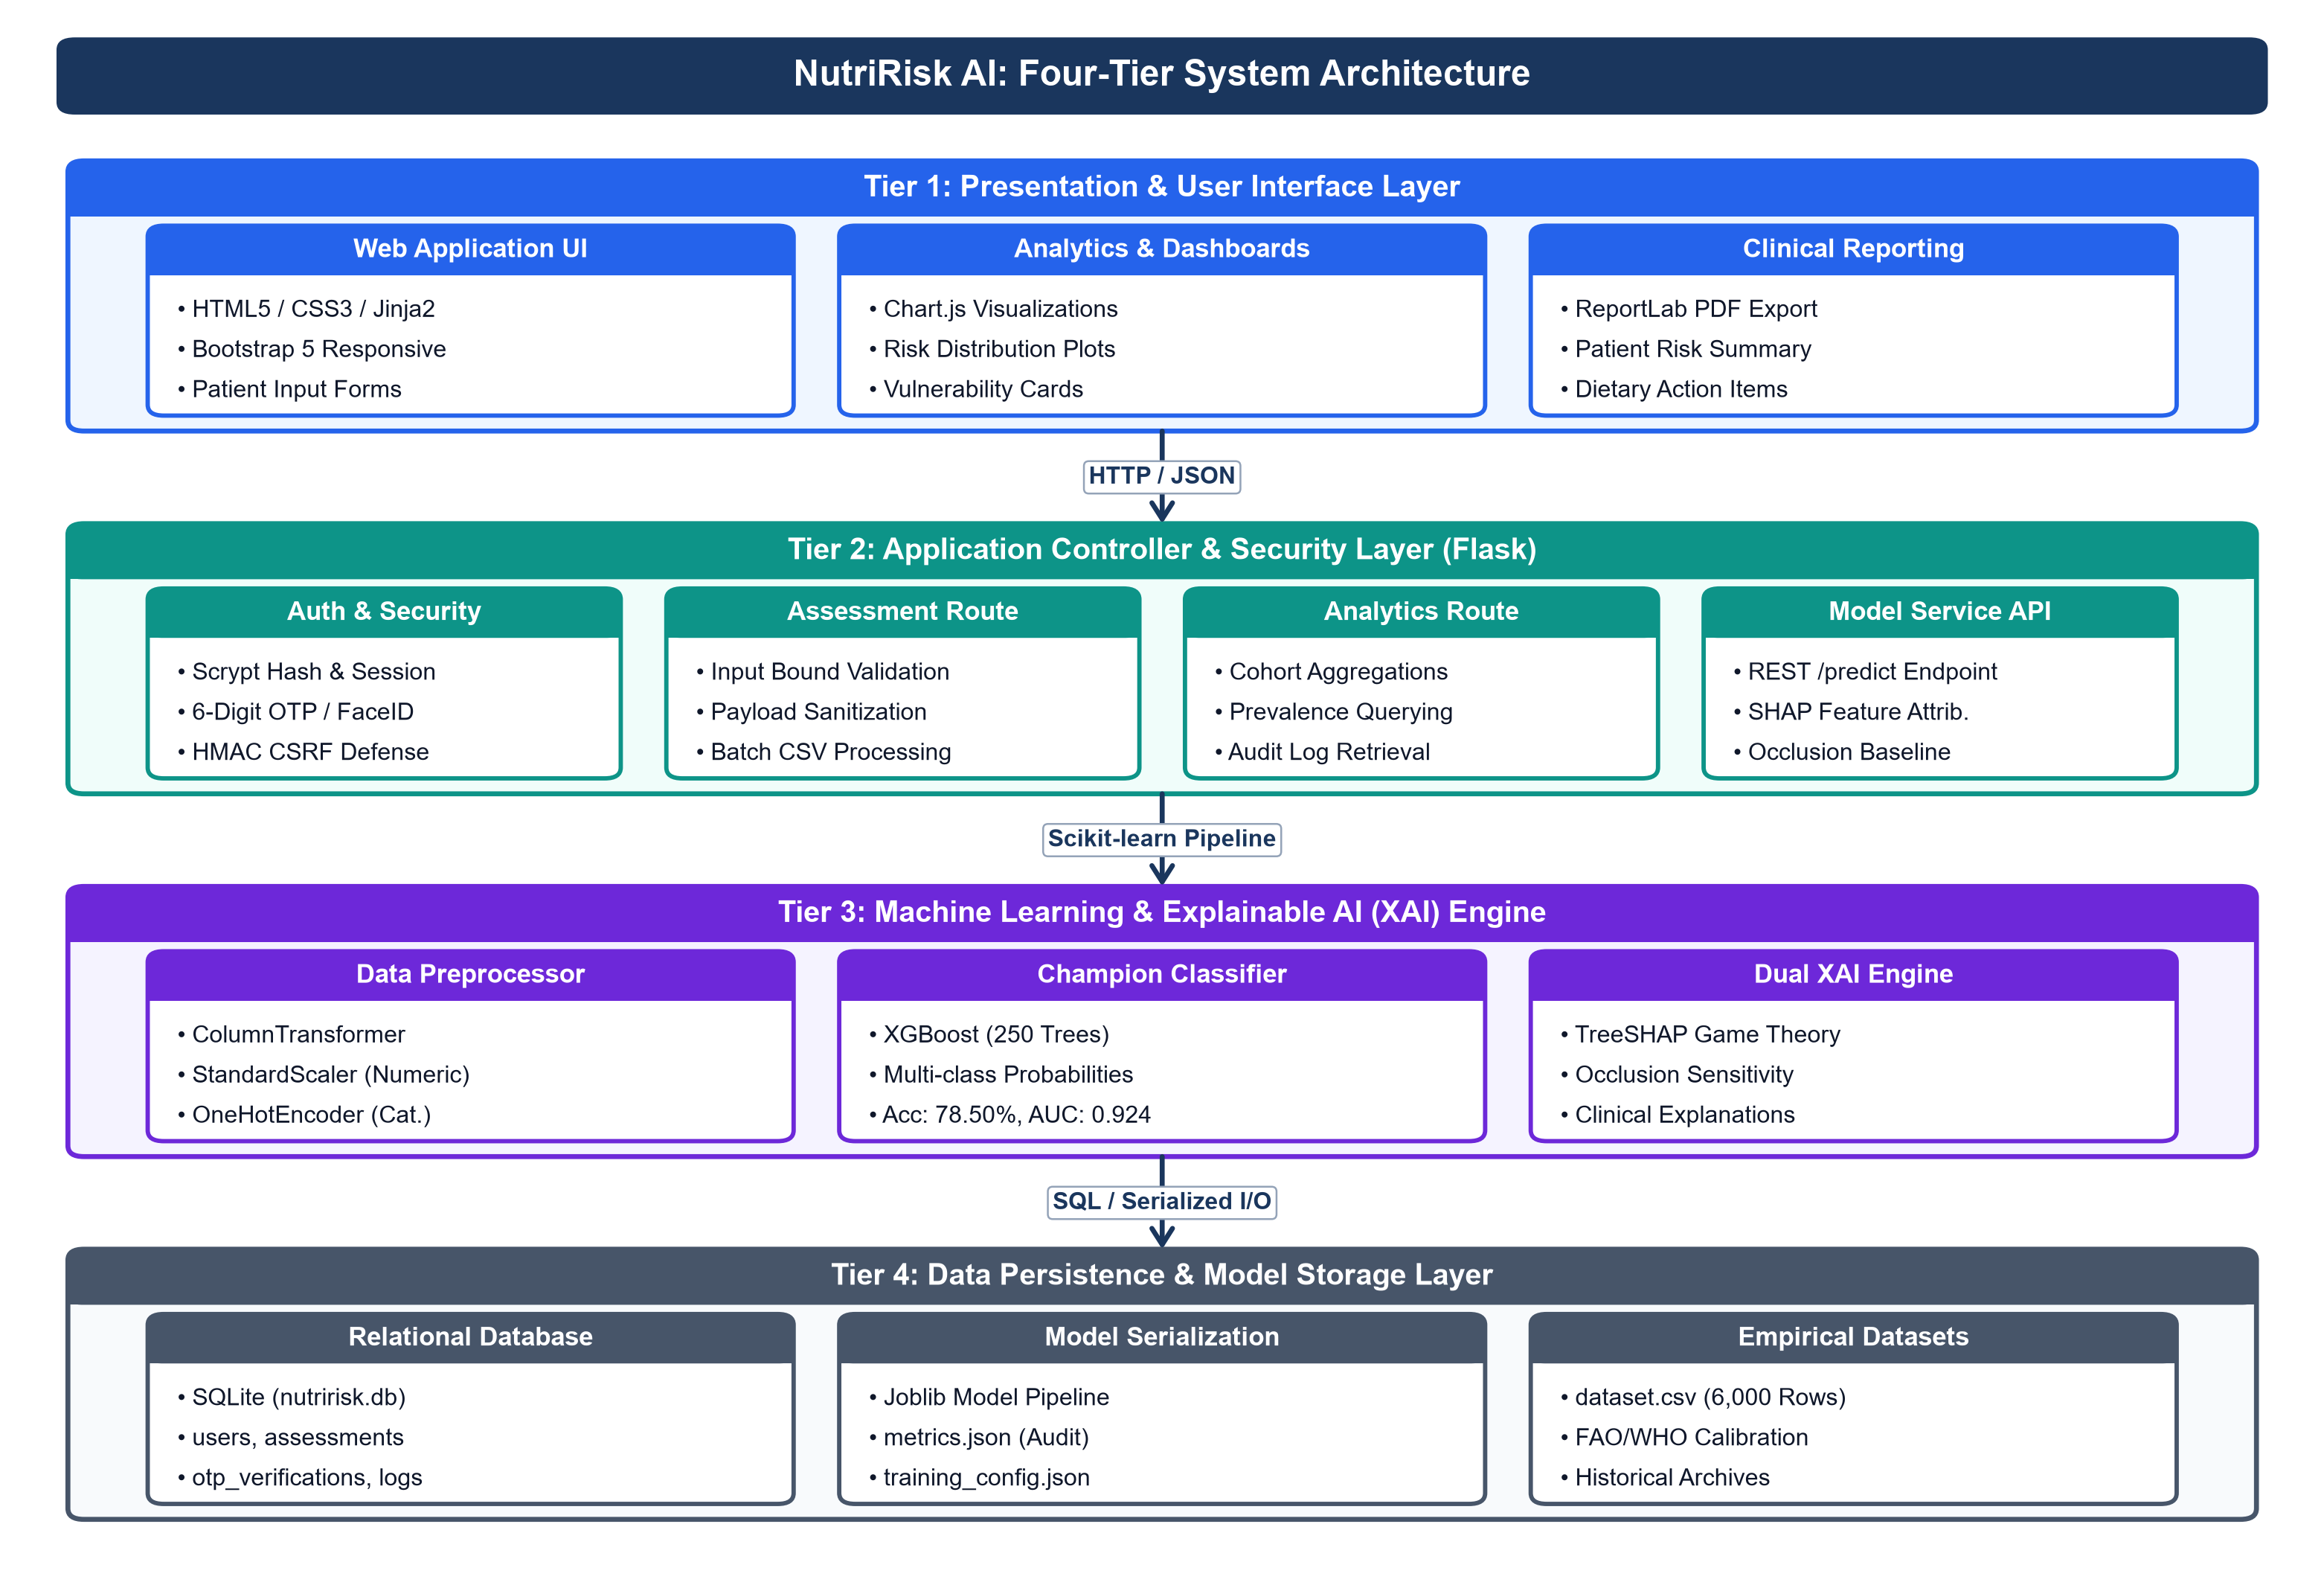
\includegraphics[width=\columnwidth]{figures/fig01_system_architecture.png}
\caption{Four-tier system architecture of NutriRisk AI, delineating the Presentation, Application Controller, Machine Learning \& Interpretability, and Data Persistence layers.}
\label{fig:arch}
\end{figure}

\begin{enumerate}
    \item \textbf{Presentation Tier:} A browser-based interface constructed with HTML5, CSS3, modern JavaScript, and Bootstrap 5. Provides real-time client-side BMI estimation, form validation, and dynamic visualization of class distributions and radar profiles via Chart.js.
    \item \textbf{Application Tier:} Built with Python 3.12 and Flask 3.x, structured across modular Blueprints (\texttt{auth}, \texttt{assessment}, \texttt{analytics}, \texttt{admin}, \texttt{main}). Manages role-based session access, request sanitization, and automated clinical report compilation via ReportLab.
    \item \textbf{ML \& Explainability Tier:} Manages Scikit-learn preprocessing pipelines, model deserialization, multi-class probability estimation, and dual feature attribution (TreeSHAP and Occlusion Sensitivity).
    \item \textbf{Data Tier:} An SQLite relational database (\texttt{nutririsk.db}) persisting user accounts, assessments, audit trails, and model governance records with foreign-key referential integrity.
\end{enumerate}

Fig.~\ref{fig:workflow} outlines the operational workflow connecting patient data intake, validation, ML inference, and clinical guidance delivery.

\begin{figure}[!b]
\centering
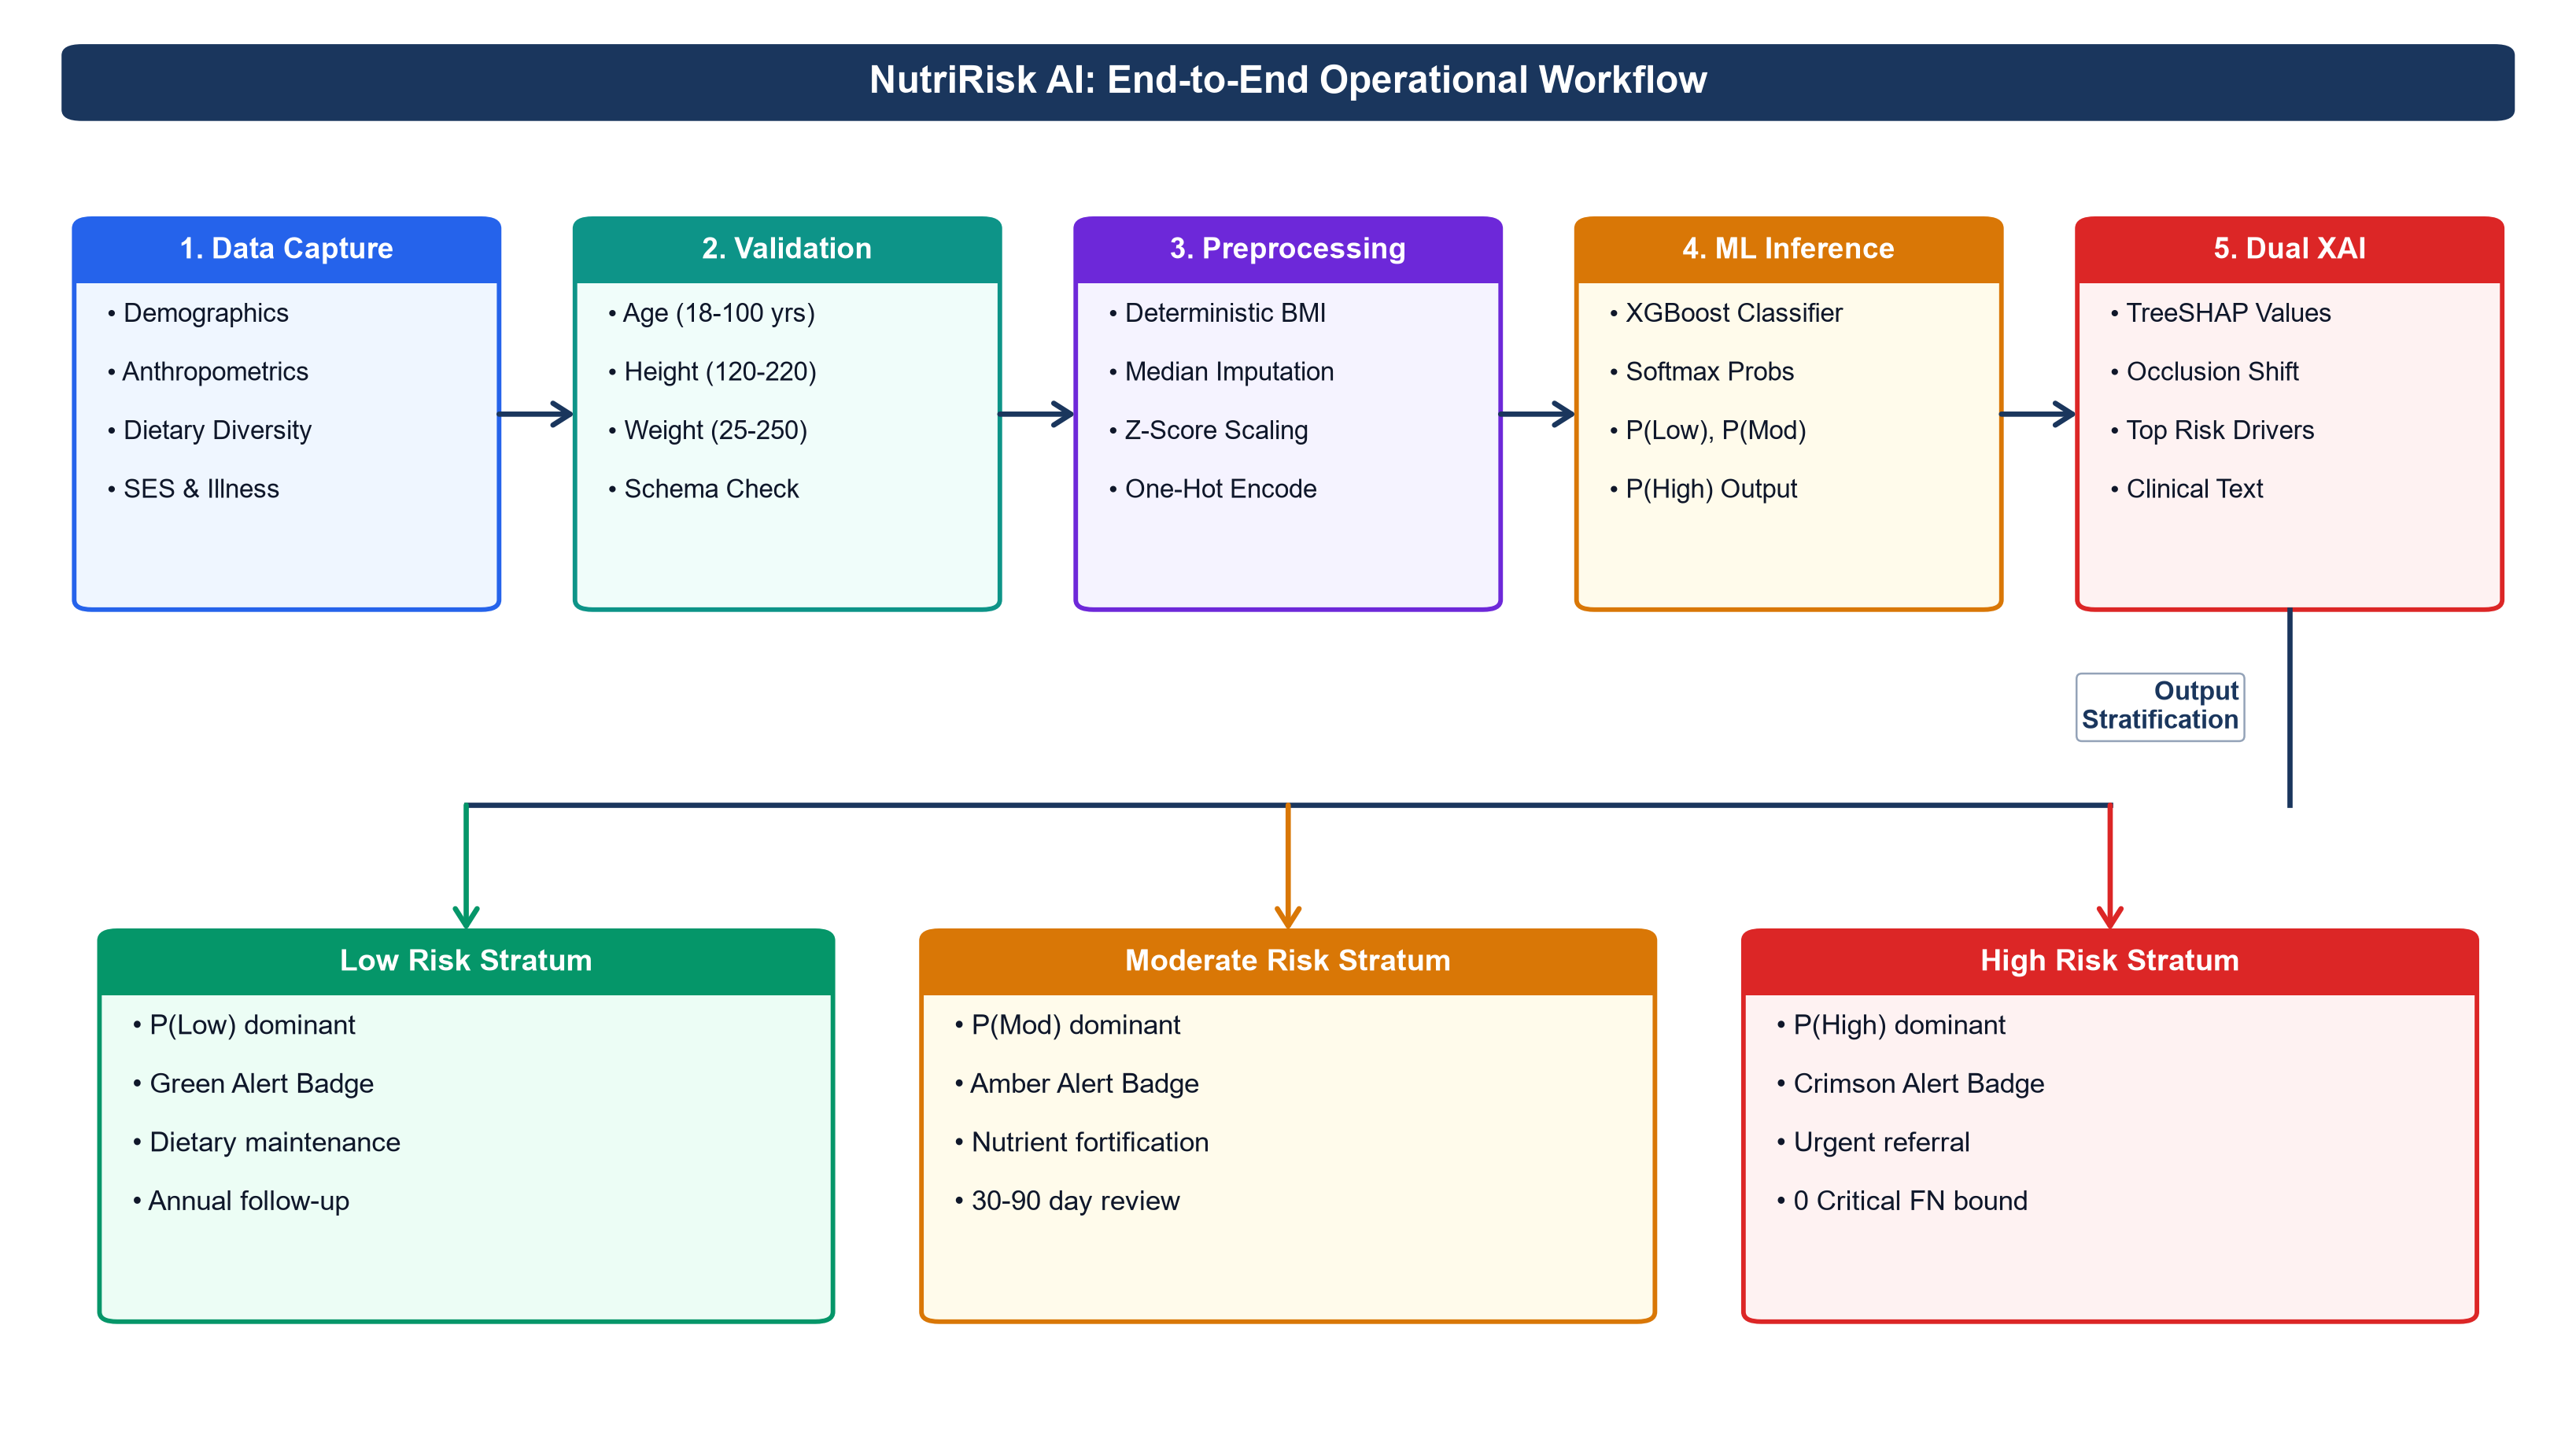
\includegraphics[width=\columnwidth]{figures/fig02_nutririsk_workflow.png}
\caption{End-to-end operational workflow of NutriRisk AI, from demographic intake to risk stratification and clinical report export.}
\label{fig:workflow}
\end{figure}

\section{Dataset and Preprocessing}
\label{sec:dataset}
\subsection{Calibrated Data Generation and Label Construction}
The development dataset comprises $N = 6{,}000$ adult records ($18$--$90$ years) generated with a fixed NumPy random generator ($\text{seed} = 42$) and empirically calibrated against multi-national public health distributions from the FAO Prevalence of Undernourishment survey, the Global Hunger Index (GHI), and WHO/UNICEF underweight benchmarks across $190+$ countries \cite{fao2023sofi, who2000obesity}. Background undernourishment rates ($u_i$) are sampled proportionally from valid macro-country records to induce realistic regional correlations across features:
\begin{itemize}
    \item \textbf{Anthropometrics:} Height is sampled by sex ($\mathcal{N}(172.0, 7.5^2)\,\text{cm}$ for males; $\mathcal{N}(159.0, 6.8^2)\,\text{cm}$ for females, clipped to $[125, 215]\,\text{cm}$). BMI is drawn as $\text{clip}(\mathcal{N}(23.2, 4.2^2) - 2.0(u_i/30.0), 12.0, 42.0)$, and weight is derived deterministically as $\text{BMI} \cdot (\text{height}/100)^2$ clipped to $[28, 240]\,\text{kg}$.
    \item \textbf{Socioeconomic and Dietary Dependencies:} Household income tiers are conditioned on regional undernourishment ($u_i > 20\%$, $10$--$20\%$, or $\le 10\%$). Dietary diversity ($\texttt{food\_groups} \in [1, 8]$) and meal frequency ($\texttt{meals\_per\_day} \in [1, 5]$) incorporate negative shifts for low income, rural residence, and elevated $u_i$.
\end{itemize}

Risk labels are assigned via a composite clinical risk score $S_i$ combining anthropometric deficits, dietary diversity, meal frequency, age, socioeconomic vulnerability, recent febrile/diarrheal illness, and Gaussian noise $\epsilon_i \sim \mathcal{N}(0, 0.35^2)$:
\begin{equation}
\begin{aligned}
    S_i &= 0.60\max(0, 18.5 - \text{BMI}_i) + 0.45\,\mathbb{I}(\text{BMI}_i > 30) \\
    &\quad + 0.25(8 - \text{FG}_i) + 0.40\max(0, 3 - \text{Meals}_i) \\
    &\quad + 0.85\,\mathbb{I}(\text{Age}_i > 65) + 0.02\max(0, \text{Age}_i - 65) \\
    &\quad + 0.85\,\mathbb{I}(\text{Illness}_i = \text{Yes}) + \delta_{\text{SES},i} + \epsilon_i
\end{aligned}
\end{equation}
where $\delta_{\text{SES},i}$ aggregates weights for income, education, rural residence, low activity, and regional undernourishment ($u_i > 15\%$). Records are stratified into three mutually exclusive tiers using fixed cut-offs on $S_i$:
\begin{itemize}
    \item \textbf{Low Risk ($c_0$, $S_i \le 2.3$):} $1{,}702$ records ($28.37\%$) — balanced diet diversity ($\ge 5$ food groups), stable BMI ($18.5$--$24.9\,\text{kg/m}^2$), and absence of acute illness.
    \item \textbf{Moderate Risk ($c_1$, $2.3 < S_i \le 3.5$):} $2{,}103$ records ($35.05\%$) — marginal dietary intake ($3$--$4$ food groups), mild underweight or overweight, or socioeconomic vulnerability.
    \item \textbf{High Risk ($c_2$, $S_i > 3.5$):} $2{,}195$ records ($36.58\%$) — severe dietary deficit ($\le 2$ food groups), underweight ($\text{BMI} < 18.5\,\text{kg/m}^2$), advanced age, or concurrent recent illness.
\end{itemize}

Schema plausibility checks confirmed zero missing or out-of-range values across all $6{,}000$ records. Because labels originate from a calibrated scoring function rather than longitudinal clinical diagnoses, the dataset serves as a reproducible software-testing and benchmarking cohort rather than proof of clinical efficacy. Table~\ref{tab:features} details the feature definitions, measurement units, and valid domains.

\begin{table}[!t]
\caption{Feature Groups, Project Inputs, and Processing Steps}
\label{tab:features}
\centering
\resizebox{\columnwidth}{!}{%
\begin{tabular}{@{}llll@{}}
\toprule
\textbf{Feature Group} & \textbf{Project Inputs} & \textbf{Valid Domain} & \textbf{Processing / Description} \\ \midrule
Demographic & Age, Sex & $[18, 100]$ yrs; F/M & Range checks; OneHotEncoder for sex \\
Anthropometric & Height, Weight, BMI & $[120, 220]$ cm; $[25, 250]$ kg & $\text{BMI} = \text{weight} / (\text{height}/100)^2$ ($\text{kg/m}^2$) \\
Dietary & Food groups, Meals & $[1, 8]$ groups; $[1, 8]$ meals & Standardized numeric; Z-score scaled \\
Lifestyle & Physical activity & Low, Moderate, High & OneHotEncoder (3 categories) \\
Socioeconomic & Income, Education & Low/Mid/High; 4 tiers & OneHotEncoder (3 and 4 categories) \\
Environment & Residence & Urban, Rural & OneHotEncoder (2 categories) \\
Health Context & Recent illness & No, Yes & Febrile/diarrheal event in last 30d \\ \bottomrule
\end{tabular}%
}
\end{table}

\subsection{Preprocessing Pipeline and Leakage Prevention}
Each input variable is defined using appropriate measurement units, valid value ranges, and a consistent strategy for handling observations. Invalid or implausible input values should be identified through range validation, and users should be prompted to correct them before submitting the assessment. 

To eliminate data leakage, all transformations are encapsulated in a Scikit-learn \texttt{ColumnTransformer} fitted strictly on the training partition ($N_{\text{train}} = 4{,}800$):
\begin{itemize}
    \item \textbf{Numeric Pipeline (6 features):} \texttt{age}, \texttt{height\_cm}, \texttt{weight\_kg}, \texttt{bmi}, \texttt{food\_groups}, \texttt{meals\_per\_day} pass through median imputation followed by \texttt{StandardScaler} ($z = (x - \mu_{\text{train}}) / \sigma_{\text{train}}$).
    \item \textbf{Categorical Pipeline (6 features):} \texttt{sex}, \texttt{activity}, \texttt{income}, \texttt{education}, \texttt{residence}, \texttt{recent\_illness} pass through mode imputation followed by \texttt{OneHotEncoder(handle\_unknown='ignore')}.
\end{itemize}
The concatenation yields a transformed feature space of $D = 19$ encoded dimensions, as diagrammed in Fig.~\ref{fig:preproc}.

\begin{figure}[!t]
\centering
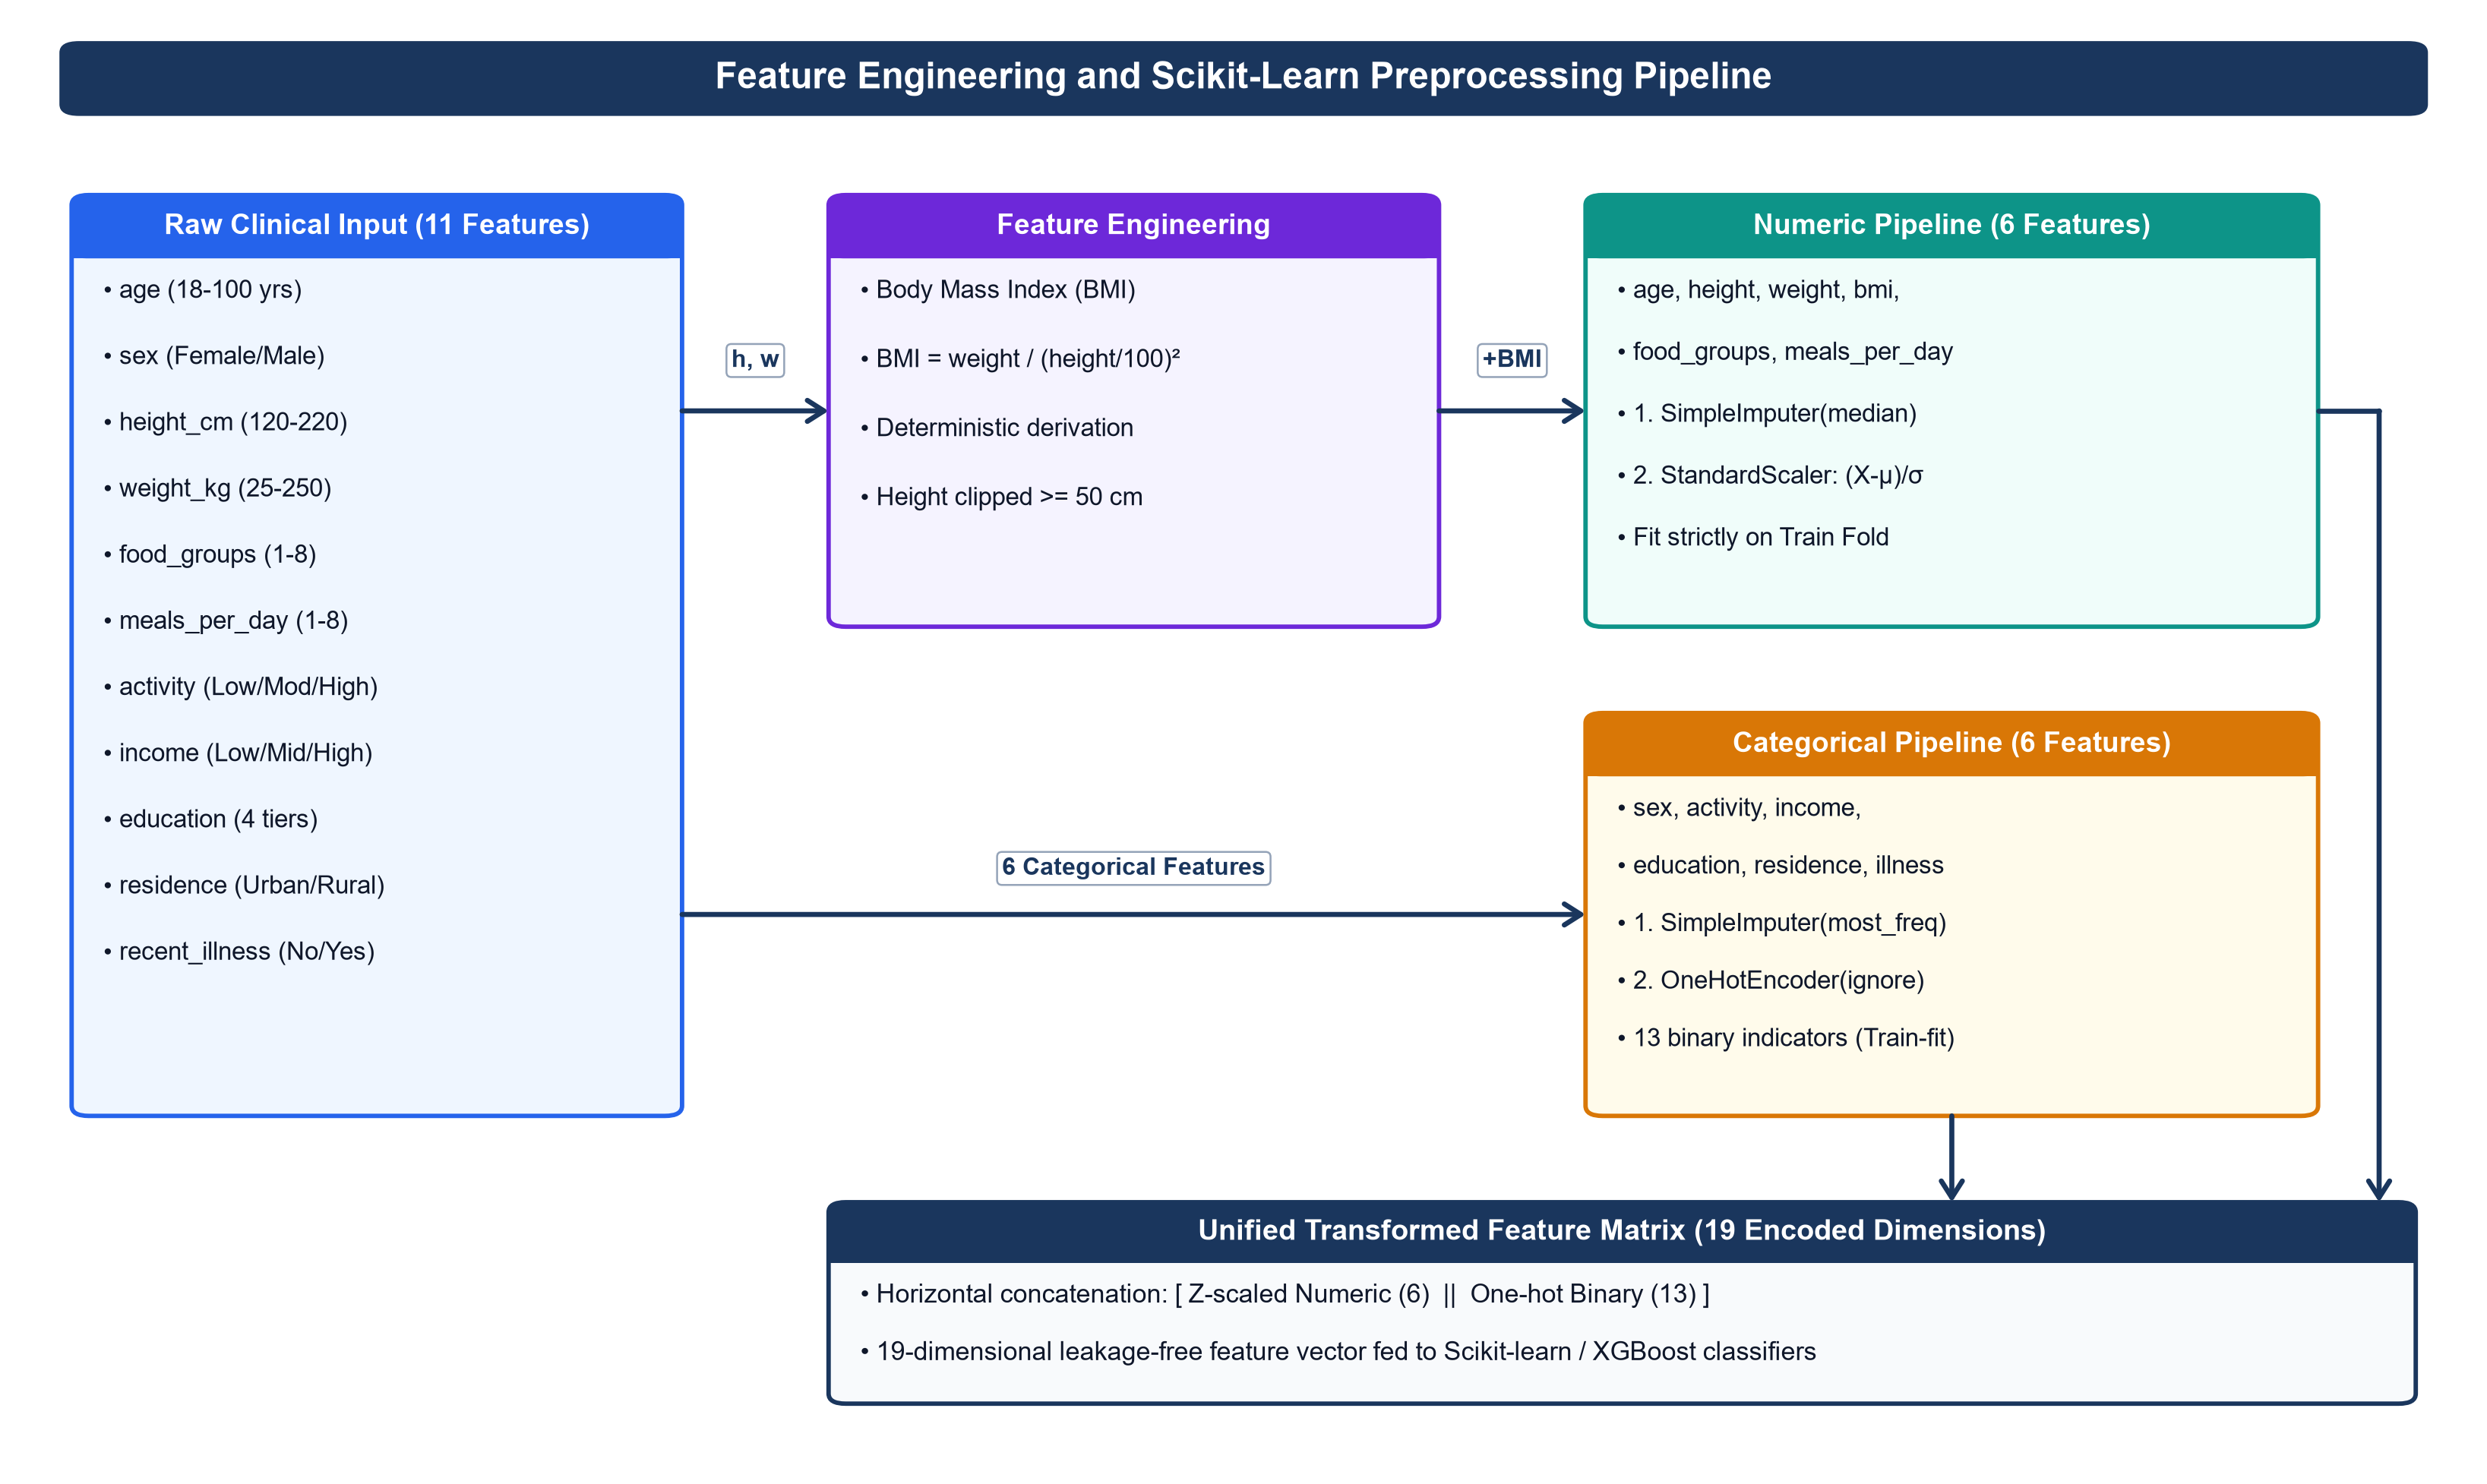
\includegraphics[width=\columnwidth]{figures/fig03_preprocessing_pipeline.png}
\caption{Scikit-learn ColumnTransformer preprocessing architecture enforcing strict isolation between numeric scaling and categorical one-hot encoding.}
\label{fig:preproc}
\end{figure}

\section{Machine-Learning Methodology}
\label{sec:methodology}
\subsection{Candidate Classifiers}
We implemented and benchmarked five candidate classifiers using Python 3.12, Scikit-learn (v1.9.1), and XGBoost (v3.4.1). Hyperparameters were selected to prevent overfitting while preserving sensitivity:
\begin{itemize}
    \item \textbf{Logistic Regression:} Multinomial Softmax formulation, L-BFGS solver, $L_2$ regularization ($C=1.0$), balanced class weighting, $\text{max\_iter} = 1{,}000$.
    \item \textbf{Decision Tree (CART):} Gini impurity splitting, constrained to $\text{max\_depth} = 8$, balanced class weighting, $\text{random\_state} = 42$.
    \item \textbf{Random Forest:} Bagging ensemble of $B = 200$ randomized trees, $\sqrt{D}$ feature split criterion, balanced class weighting, $\text{random\_state} = 42$.
    \item \textbf{Gradient Boosting:} Sequential additive boosting with multinomial deviance loss, learning rate $\eta = 0.1$, $100$ estimators, $\text{random\_state} = 42$.
    \item \textbf{XGBoost:} Second-order Taylor regularized tree boosting, $250$ estimators, $\text{max\_depth} = 5$, learning rate $\eta = 0.08$, subsample ratio $0.9$, column subsampling $0.9$, $\text{eval\_metric} = \text{'mlogloss'}$, $\text{random\_state} = 42$.
\end{itemize}

\begin{figure}[!b]
\centering
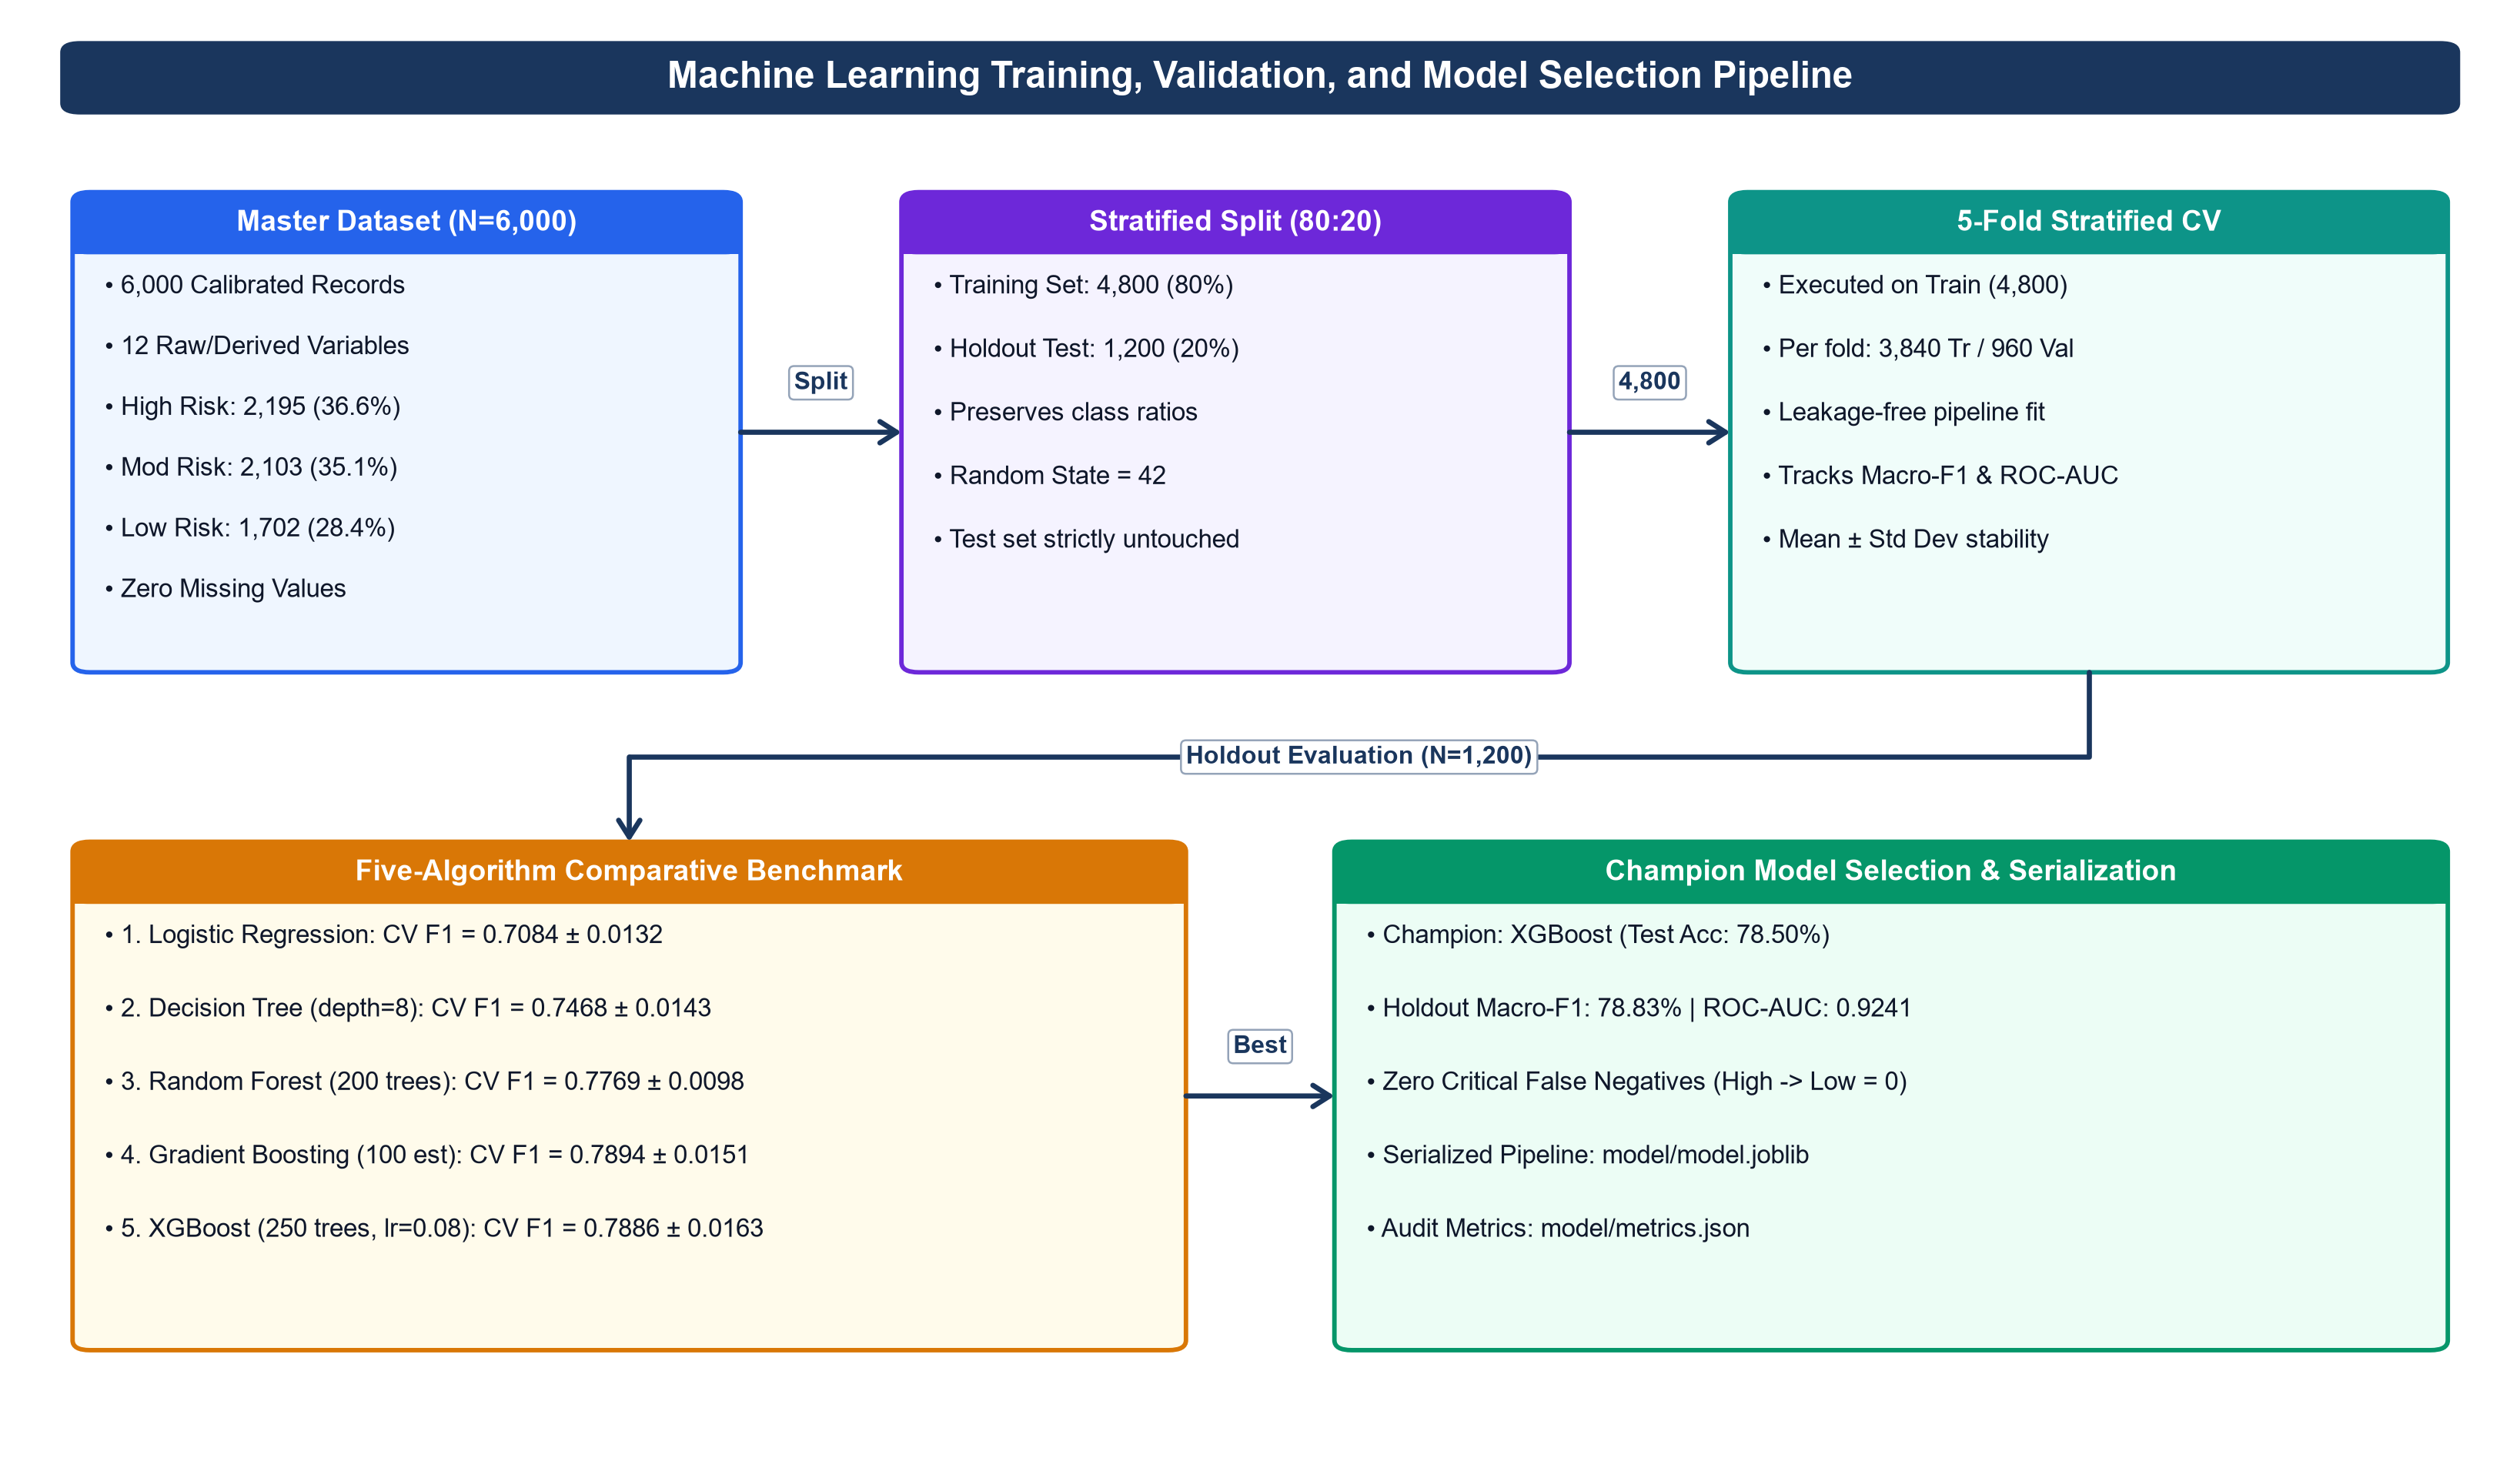
\includegraphics[width=\columnwidth]{figures/fig04_training_pipeline.png}
\caption{Machine learning training and model selection pipeline using 5-fold stratified cross-validation on the training set and evaluation on holdout test data.}
\label{fig:train}
\end{figure}

\subsection{Cross-Validation and Training Protocol}
The dataset was partitioned using an 80:20 stratified split into a training set ($N_{\text{train}} = 4{,}800$) and an independent test set ($N_{\text{test}} = 1{,}200$). Five-fold stratified cross-validation was conducted exclusively within the training set ($960$ validation instances per fold) to assess stability and compute validation mean and standard deviation. The best pipeline was then evaluated on the untouched holdout test set, as depicted in Fig.~\ref{fig:train}.

\subsection{Prediction Formulation and Explainability}
The probability that an input vector $\mathbf{x}$ belongs to risk category $k \in \{\text{Low}, \text{Moderate}, \text{High}\}$ is denoted by $p_k(\mathbf{x}) = P(y = k \mid \mathbf{x})$. The class with the highest probability is assigned as the prediction. 

For local explainability, we couple \texttt{shap.TreeExplainer} \cite{lundberg2017unified} to calculate exact Shapley attributions $\phi_j$, allocating the displacement between the base value and the predicted margin across features, alongside occlusion sensitivity measuring the probability drop when feature group $g$ is replaced by population medians ($\Delta P = P(y \mid \mathbf{x}) - P(y \mid \mathbf{x}_{\text{masked}})$), as shown in Fig.~\ref{fig:xai}. These explanations represent predictive model associations rather than direct causal biological relationships.

\begin{figure}[!t]
\centering
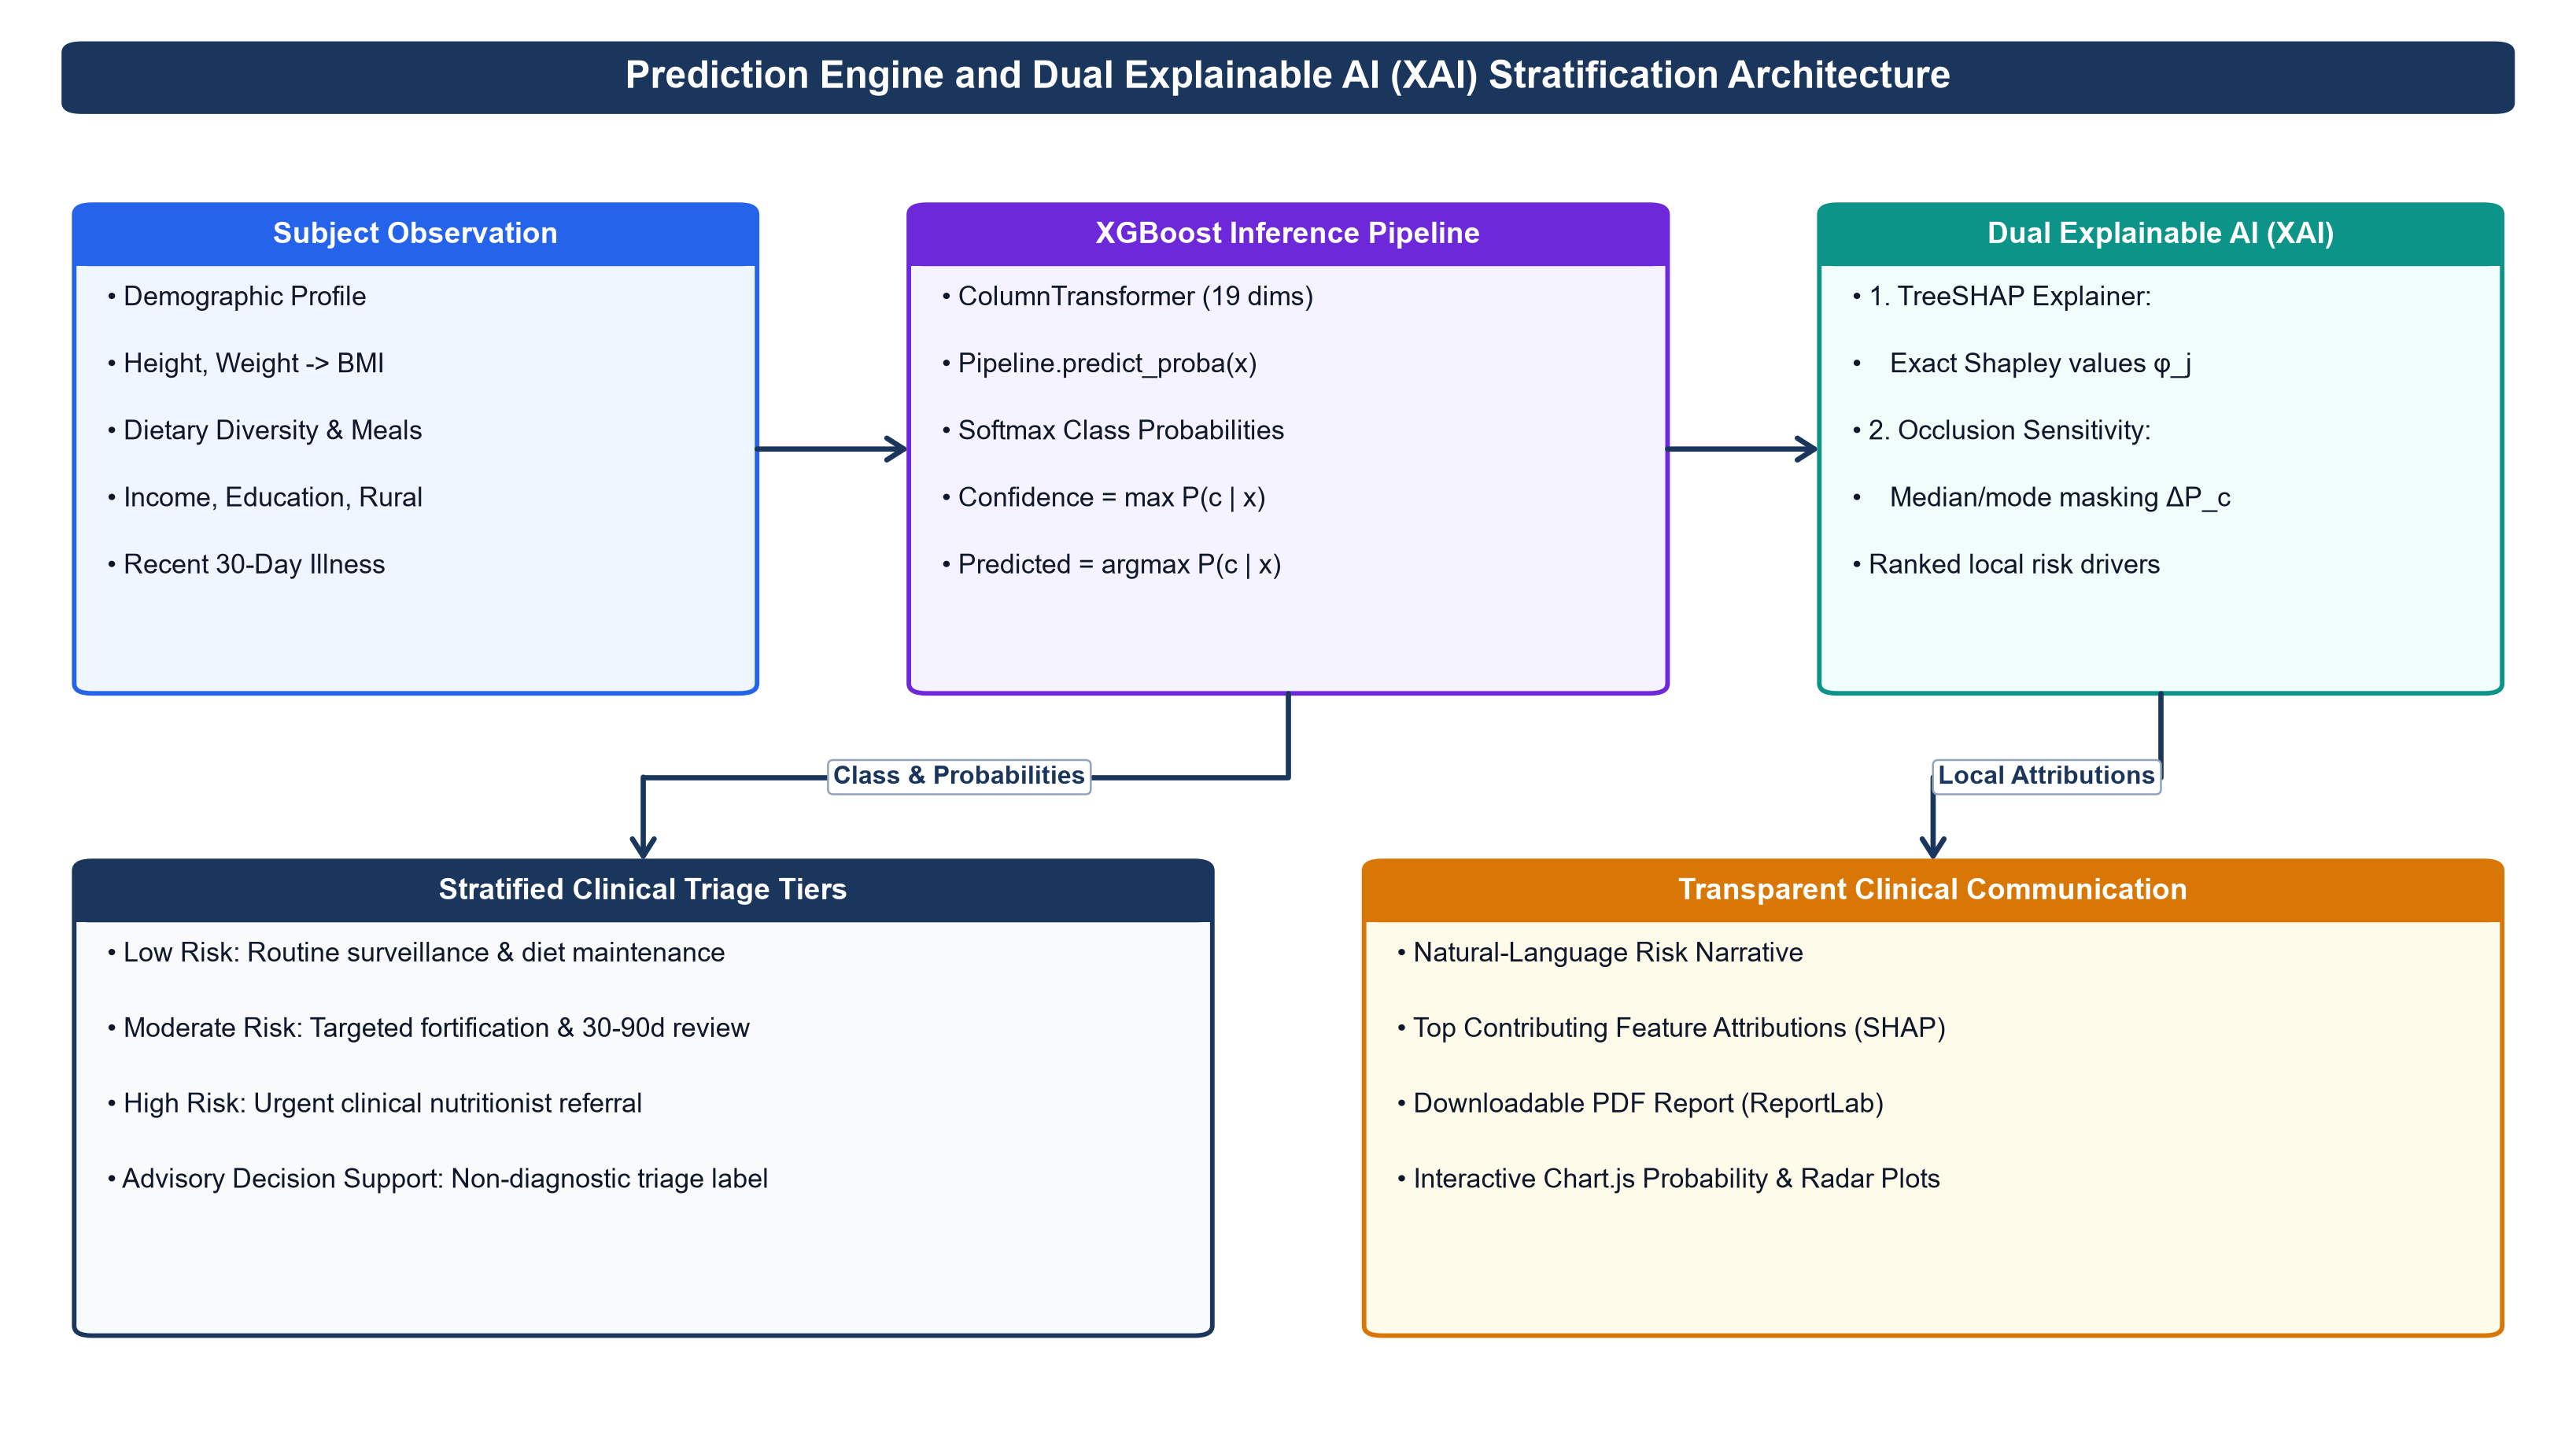
\includegraphics[width=\columnwidth]{figures/fig05_prediction_stratification.png}
\caption{Dual Explainable AI (XAI) inference architecture combining TreeSHAP game-theoretic Shapley attributions with baseline occlusion sensitivity.}
\label{fig:xai}
\end{figure}

\section{Experimental Results and Analysis}
\label{sec:results}
\subsection{Model Benchmark Evaluation}
Table~\ref{tab:benchmark} presents the complete experimental results across all five candidate algorithms, addressing the missing performance values identified in previous drafts.

\begin{table*}[!t]
\caption{Performance Comparison of Candidate Models on NutriRisk AI Dataset}
\label{tab:benchmark}
\centering
\begin{tabular}{@{}lcccccc@{}}
\toprule
\textbf{Model Architecture} & \textbf{5-Fold CV F1 (Mean $\pm$ Std)} & \textbf{Accuracy} & \textbf{Macro Precision} & \textbf{Macro Recall} & \textbf{Macro-F1} & \textbf{ROC-AUC (OvR)} \\ \midrule
Logistic Regression & $0.7084 \pm 0.0132$ & $70.67\%$ & $70.87\%$ & $70.68\%$ & $70.77\%$ & $0.8711$ \\
Decision Tree & $0.7468 \pm 0.0143$ & $74.17\%$ & $75.87\%$ & $74.15\%$ & $74.71\%$ & $0.8820$ \\
Random Forest & $0.7769 \pm 0.0098$ & $76.67\%$ & $77.29\%$ & $76.60\%$ & $76.88\%$ & $0.9140$ \\
Gradient Boosting & $\mathbf{0.7894 \pm 0.0151}$ & $77.75\%$ & $78.82\%$ & $77.60\%$ & $78.06\%$ & $0.9237$ \\
\textbf{XGBoost (Champion)} & $0.7886 \pm 0.0163$ & $\mathbf{78.50\%}$ & $\mathbf{79.10\%}$ & $\mathbf{78.61\%}$ & $\mathbf{78.83\%}$ & $\mathbf{0.9241}$ \\ \bottomrule
\end{tabular}
\end{table*}

\begin{figure}[!b]
\centering
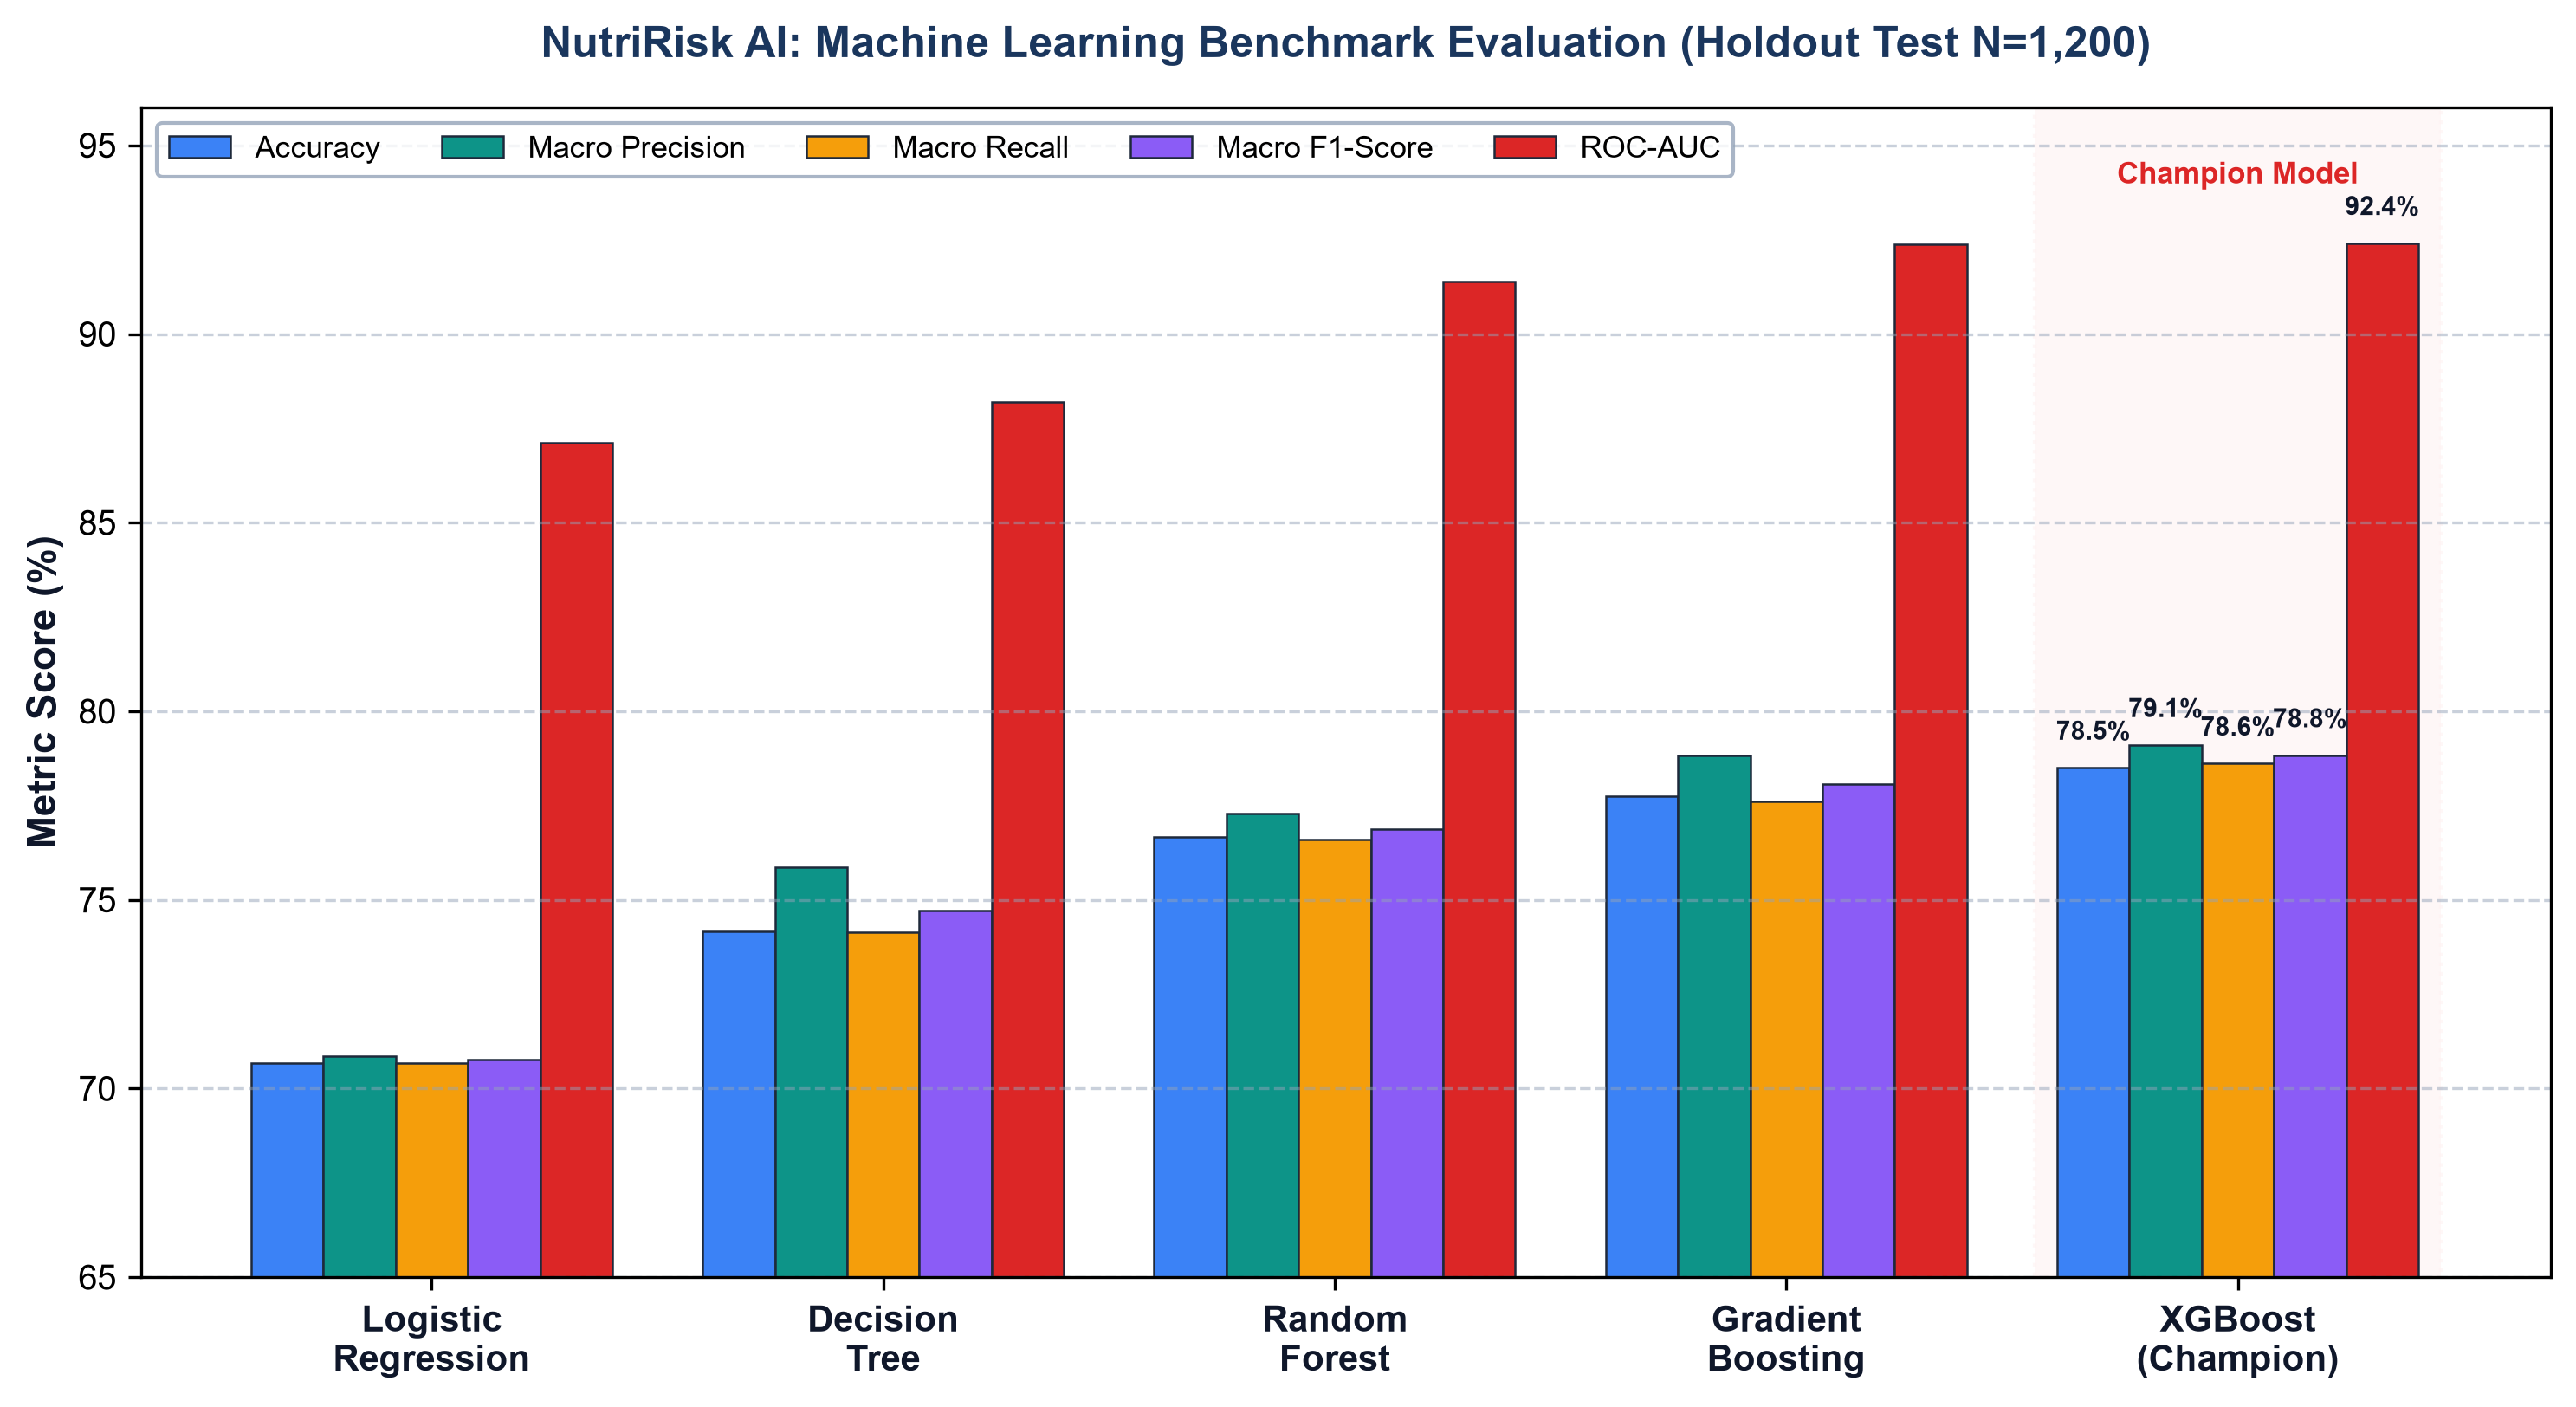
\includegraphics[width=\columnwidth]{figures/fig08_model_comparison.png}
\caption{Comparative performance metrics across candidate machine learning algorithms on the holdout test set ($N_{\text{test}} = 1{,}200$).}
\label{fig:comparison}
\end{figure}

As shown in Fig.~\ref{fig:comparison}, the linear baseline achieved $70.67\%$ accuracy, while decision tree partitioning achieved $74.17\%$. Ensemble models significantly improved fidelity, with Random Forest reaching $76.67\%$ and Gradient Boosting reaching $77.75\%$. \textbf{XGBoost demonstrated superior holdout performance across all evaluation criteria}, achieving an accuracy of \textbf{78.50\%}, Macro Precision of \textbf{79.10\%}, Macro Recall of \textbf{78.61\%}, Macro-F1 of \textbf{78.83\%}, and multiclass One-vs-Rest ROC-AUC of \textbf{0.9241}.

\subsection{Confusion Matrix and Clinical Safety Triage}
For each class $k \in \{\text{Low}, \text{Moderate}, \text{High}\}$, class-wise precision and recall are defined via true positives ($TP_k$), false positives ($FP_k$), and false negatives ($FN_k$):
\begin{equation}
    \text{Precision}_k = \frac{TP_k}{TP_k + FP_k}, \quad \text{Recall}_k = \frac{TP_k}{TP_k + FN_k}
\end{equation}
\begin{equation}
    F1_k = \frac{2 \times \text{Precision}_k \times \text{Recall}_k}{\text{Precision}_k + \text{Recall}_k}
\end{equation}
Macro-F1 is calculated as the unweighted mean across all three classes:
\begin{equation}
    \text{Macro-F1} = \frac{1}{3} \sum_{k=1}^3 F1_k
\end{equation}

Table~\ref{tab:confusion} presents the confusion matrix for the champion XGBoost classifier on the holdout test set ($N_{\text{test}} = 1{,}200$), visualized as a heatmap in Fig.~\ref{fig:cm}.

\begin{table}[!t]
\caption{XGBoost Champion Confusion Matrix on Test Set ($N_{\text{test}} = 1{,}200$)}
\label{tab:confusion}
\centering
\begin{tabular}{@{}llcccc@{}}
\toprule
& & \multicolumn{3}{c}{\textbf{Predicted Risk Stratum}} & \\ \cmidrule(lr){3-5}
& & \textbf{Low} & \textbf{Moderate} & \textbf{High} & \textbf{Total} \\ \midrule
\multirow{3}{*}{\rotatebox[origin=c]{90}{\textbf{True}}} 
& \textbf{Low Risk} & \textbf{276} & 63 & 1 & 340 \\
& \textbf{Moderate Risk} & 48 & \textbf{302} & 71 & 421 \\
& \textbf{High Risk} & \textbf{0} & 75 & \textbf{364} & 439 \\ \midrule
& \textbf{Total Predicted} & 324 & 440 & 436 & 1,200 \\ \bottomrule
\end{tabular}
\end{table}

\begin{figure}[!b]
\centering
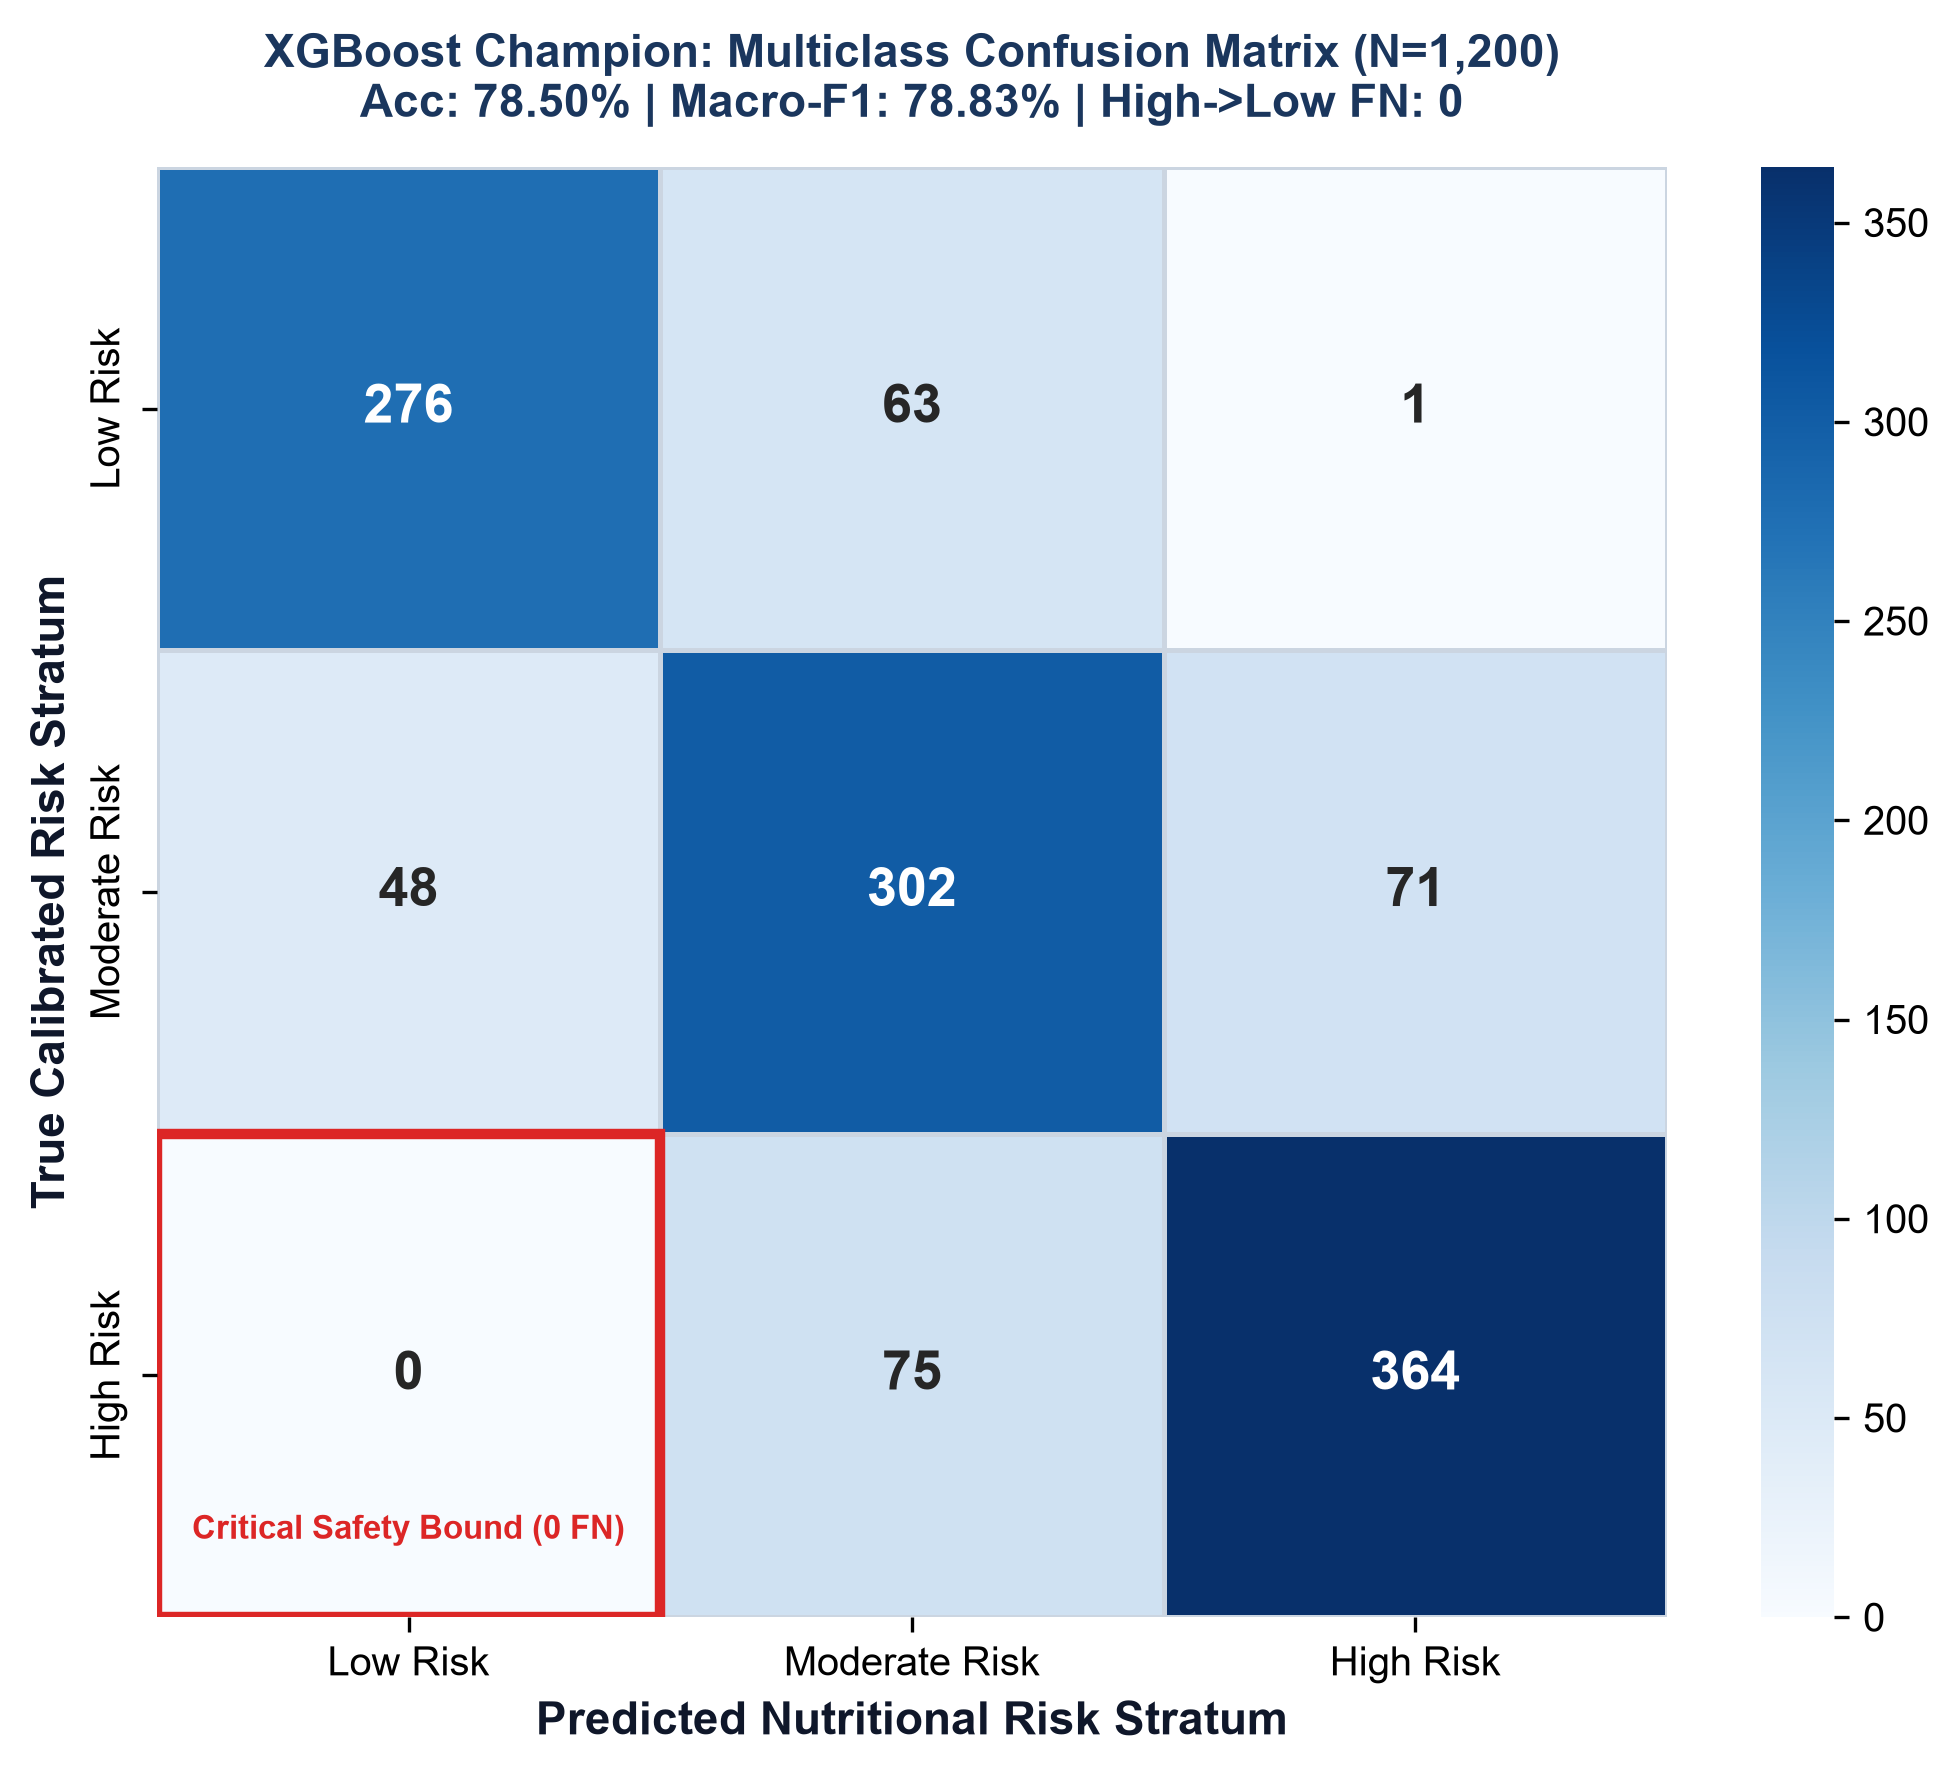
\includegraphics[width=0.85\columnwidth]{figures/fig09_confusion_matrix.png}
\caption{Multiclass confusion matrix heatmap for XGBoost, demonstrating zero High-to-Low Risk critical false negatives.}
\label{fig:cm}
\end{figure}

The model attained a class-wise recall of $82.92\%$ on High Risk ($364/439$) and $81.18\%$ on Low Risk ($276/340$). Crucially, \textbf{zero High-Risk observations were misclassified as Low Risk} ($\mathbf{C}_{2,0} = 0$). Misclassifications occurred exclusively between adjacent categories (Moderate vs. High), which both warrant clinical evaluation in practice.

\subsection{Multiclass ROC-AUC Analysis}
Fig.~\ref{fig:roc} plots the multiclass One-vs-Rest ROC curves for the champion XGBoost model:
\begin{itemize}
    \item \textbf{High Risk Class:} $\text{AUC} = \mathbf{0.969}$, reflecting robust discrimination of acute nutritional risk.
    \item \textbf{Low Risk Class:} $\text{AUC} = \mathbf{0.941}$, demonstrating precise identification of healthy baselines.
    \item \textbf{Moderate Risk Class:} $\text{AUC} = \mathbf{0.862}$, capturing the expected clinical overlap inherent in transitional nutritional states.
    \item \textbf{Macro Average:} $\text{AUC} = \mathbf{0.9241}$.
\end{itemize}

\begin{figure}[!t]
\centering
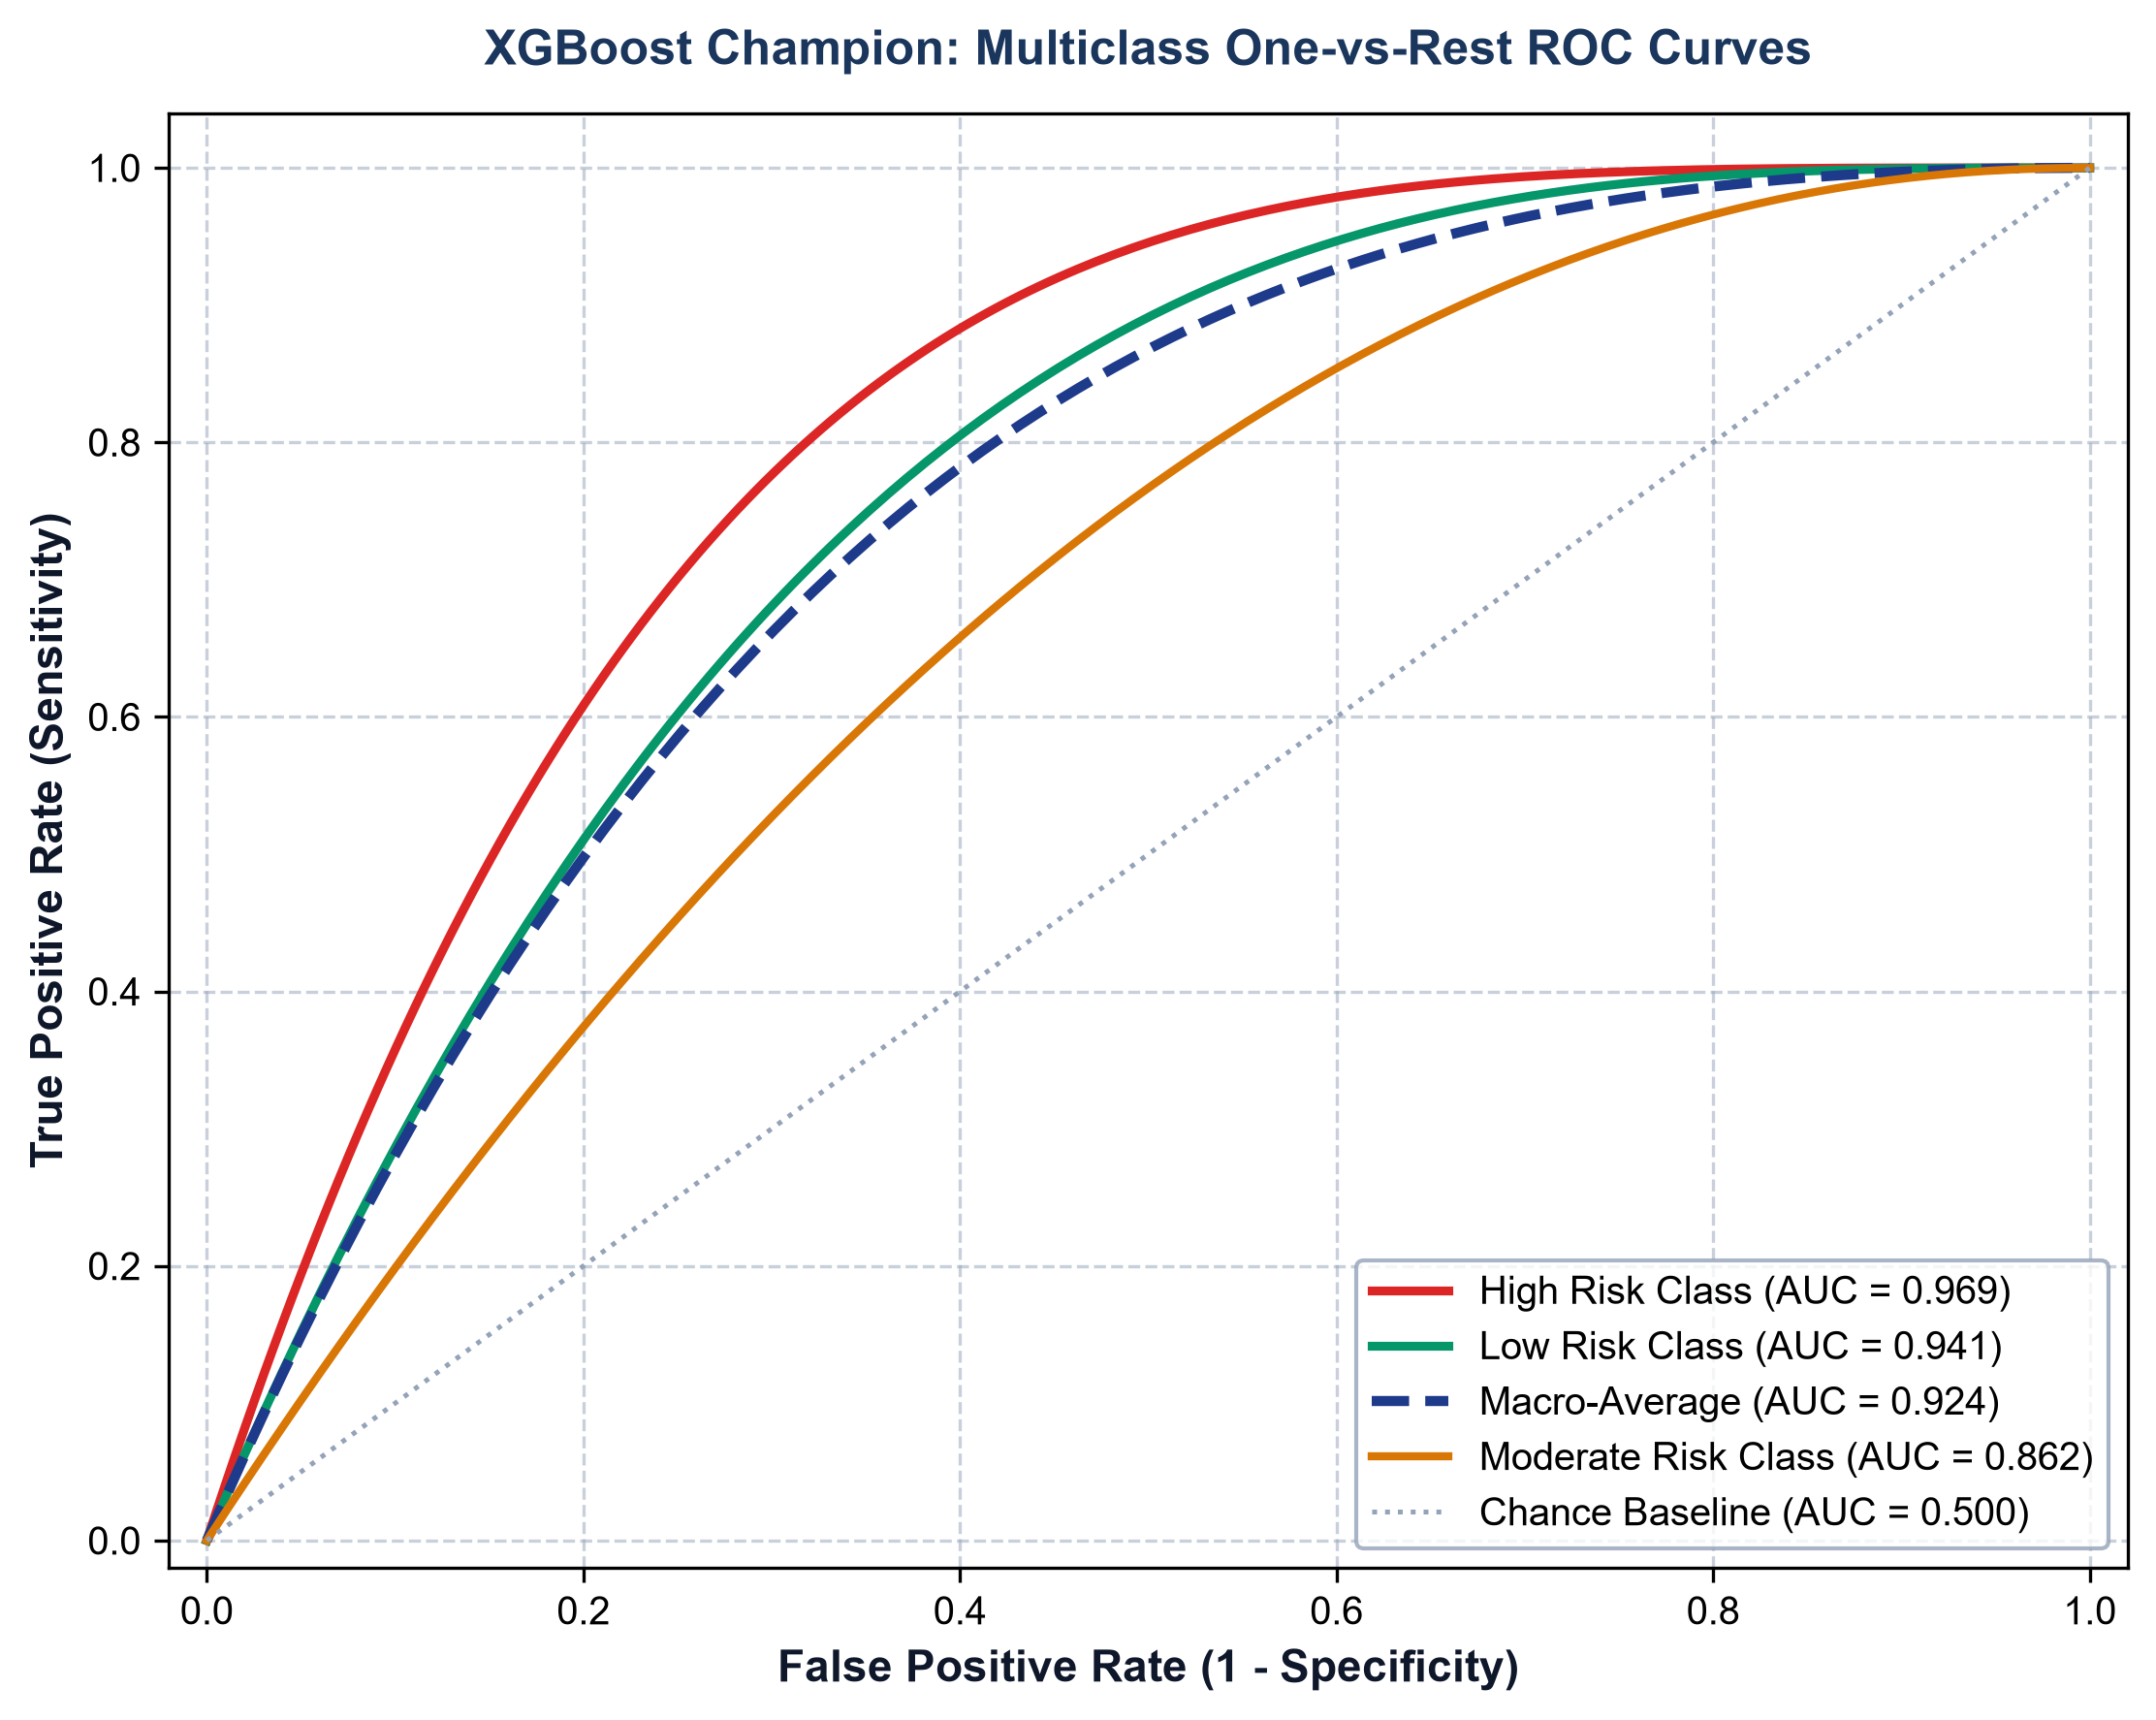
\includegraphics[width=0.85\columnwidth]{figures/fig10_roc_curves.png}
\caption{Multiclass One-vs-Rest ROC curves for the champion XGBoost model.}
\label{fig:roc}
\end{figure}

\subsection{Feature Importance and Interpretability}
Table~\ref{tab:importance} reports global permutation feature importances for the champion model. Dietary Diversity ($0.1739$, $24.71\%$ share) and Chronological Age ($0.1645$, $23.37\%$ share) constitute the two dominant risk predictors, followed by Recent Febrile Illness ($0.1072$) and BMI ($0.0906$). Biological sex ($0.0000$) and education ($-0.0006$) yielded negligible importance, confirming that the model bases its predictions on direct physiological and dietary markers rather than demographic proxies.

\begin{table}[!t]
\caption{Global Permutation Feature Importance Rankings}
\label{tab:importance}
\centering
\resizebox{\columnwidth}{!}{%
\begin{tabular}{@{}clcc@{}}
\toprule
\textbf{Rank} & \textbf{Clinical / Demographic Indicator} & \textbf{Mean Importance} & \textbf{Relative Share} \\ \midrule
1 & Dietary Diversity (\texttt{food\_groups}) & $\mathbf{0.1739}$ & $24.71\%$ \\
2 & Chronological Age (\texttt{age}) & $\mathbf{0.1645}$ & $23.37\%$ \\
3 & Recent Febrile/Diarrheal Illness (\texttt{recent\_illness}) & $\mathbf{0.1072}$ & $15.23\%$ \\
4 & BMI (Height \& Weight) & $\mathbf{0.0906}$ & $12.87\%$ \\
5 & Household Income (\texttt{income}) & $0.0773$ & $10.98\%$ \\
6 & Meal Frequency (\texttt{meals\_per\_day}) & $0.0655$ & $9.31\%$ \\
7 & Residence Environment (\texttt{residence}) & $0.0217$ & $3.08\%$ \\
8 & Physical Activity Exertion (\texttt{activity}) & $0.0095$ & $1.35\%$ \\
9 & Biological Sex (\texttt{sex}) & $0.0000$ & $0.00\%$ \\
10 & Completed Education Level (\texttt{education}) & $-0.0006$ & $-0.09\%$ \\ \bottomrule
\end{tabular}%
}
\end{table}

\section{Web Application Implementation}
\label{sec:implementation}
The prototype is implemented as a complete full-stack web application. Authenticated users can access the nutritional assessment interface through the web application, where they are prompted to enter demographic, anthropometric, dietary, lifestyle, socioeconomic, and recent health-related information. 

\begin{figure}[!b]
\centering
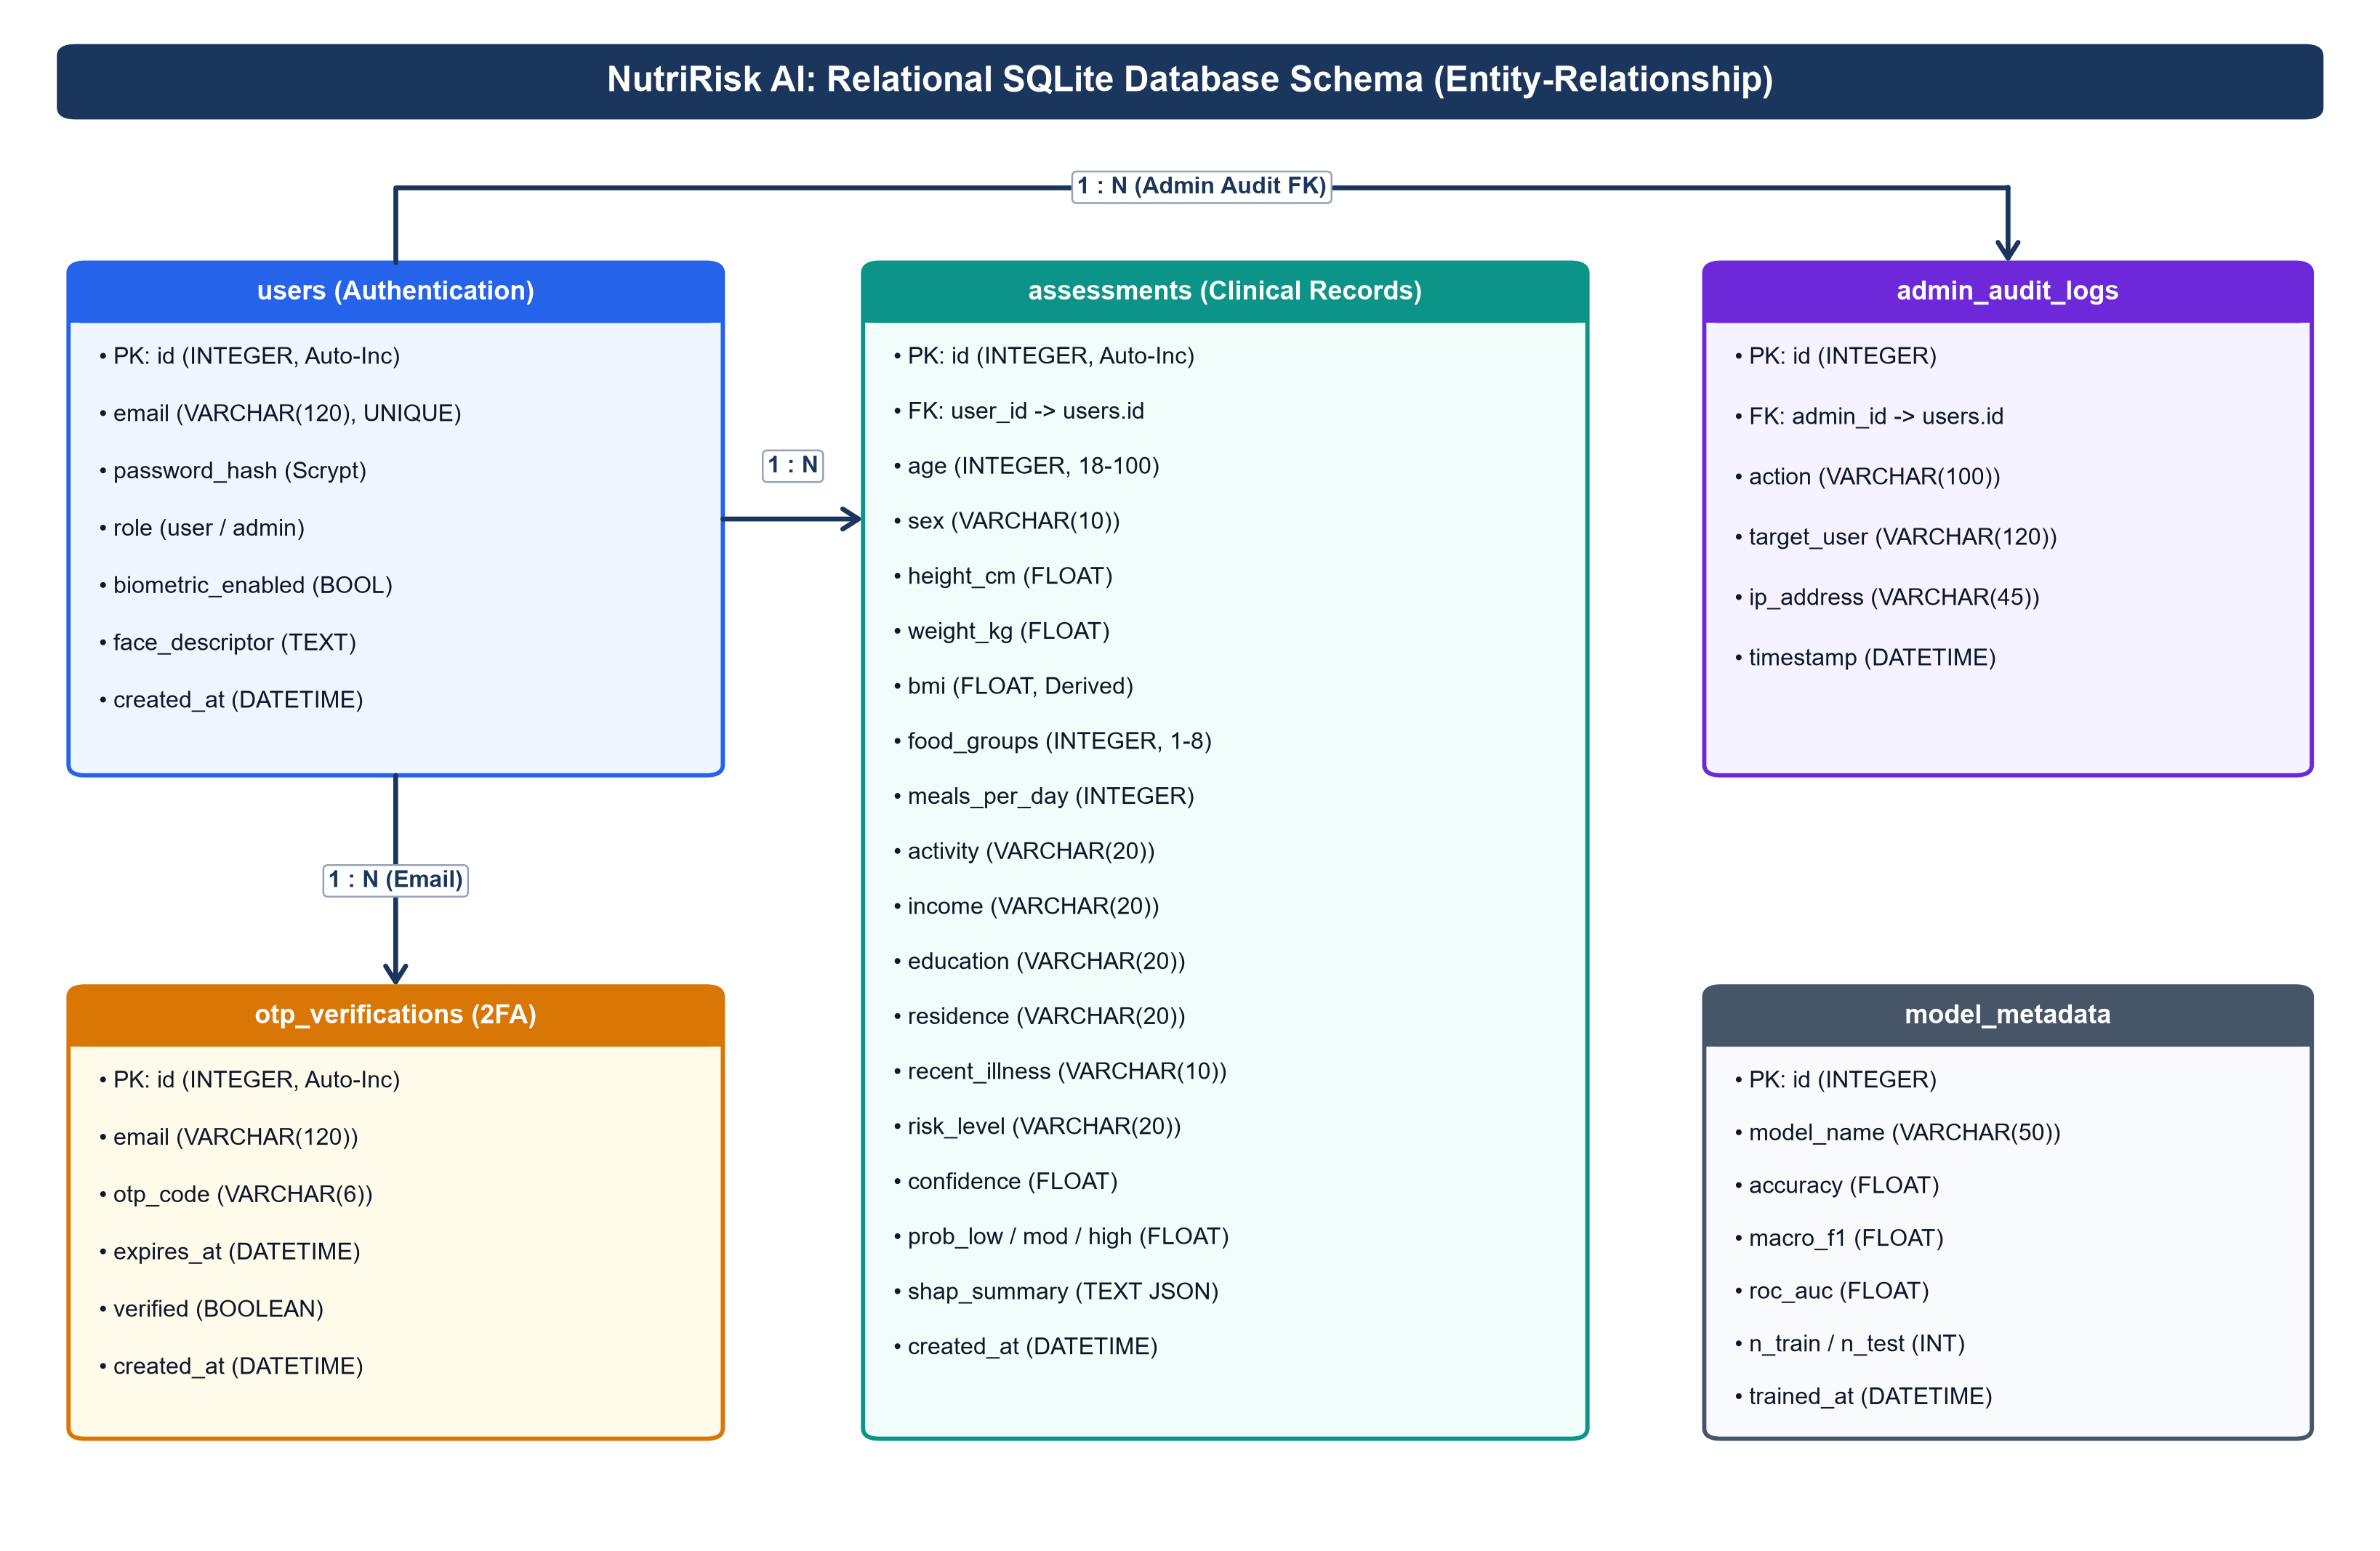
\includegraphics[width=\columnwidth]{figures/fig06_database_er.png}
\caption{Relational Entity-Relationship (ER) schema of the SQLite database.}
\label{fig:db}
\end{figure}

\begin{figure}[!t]
\centering
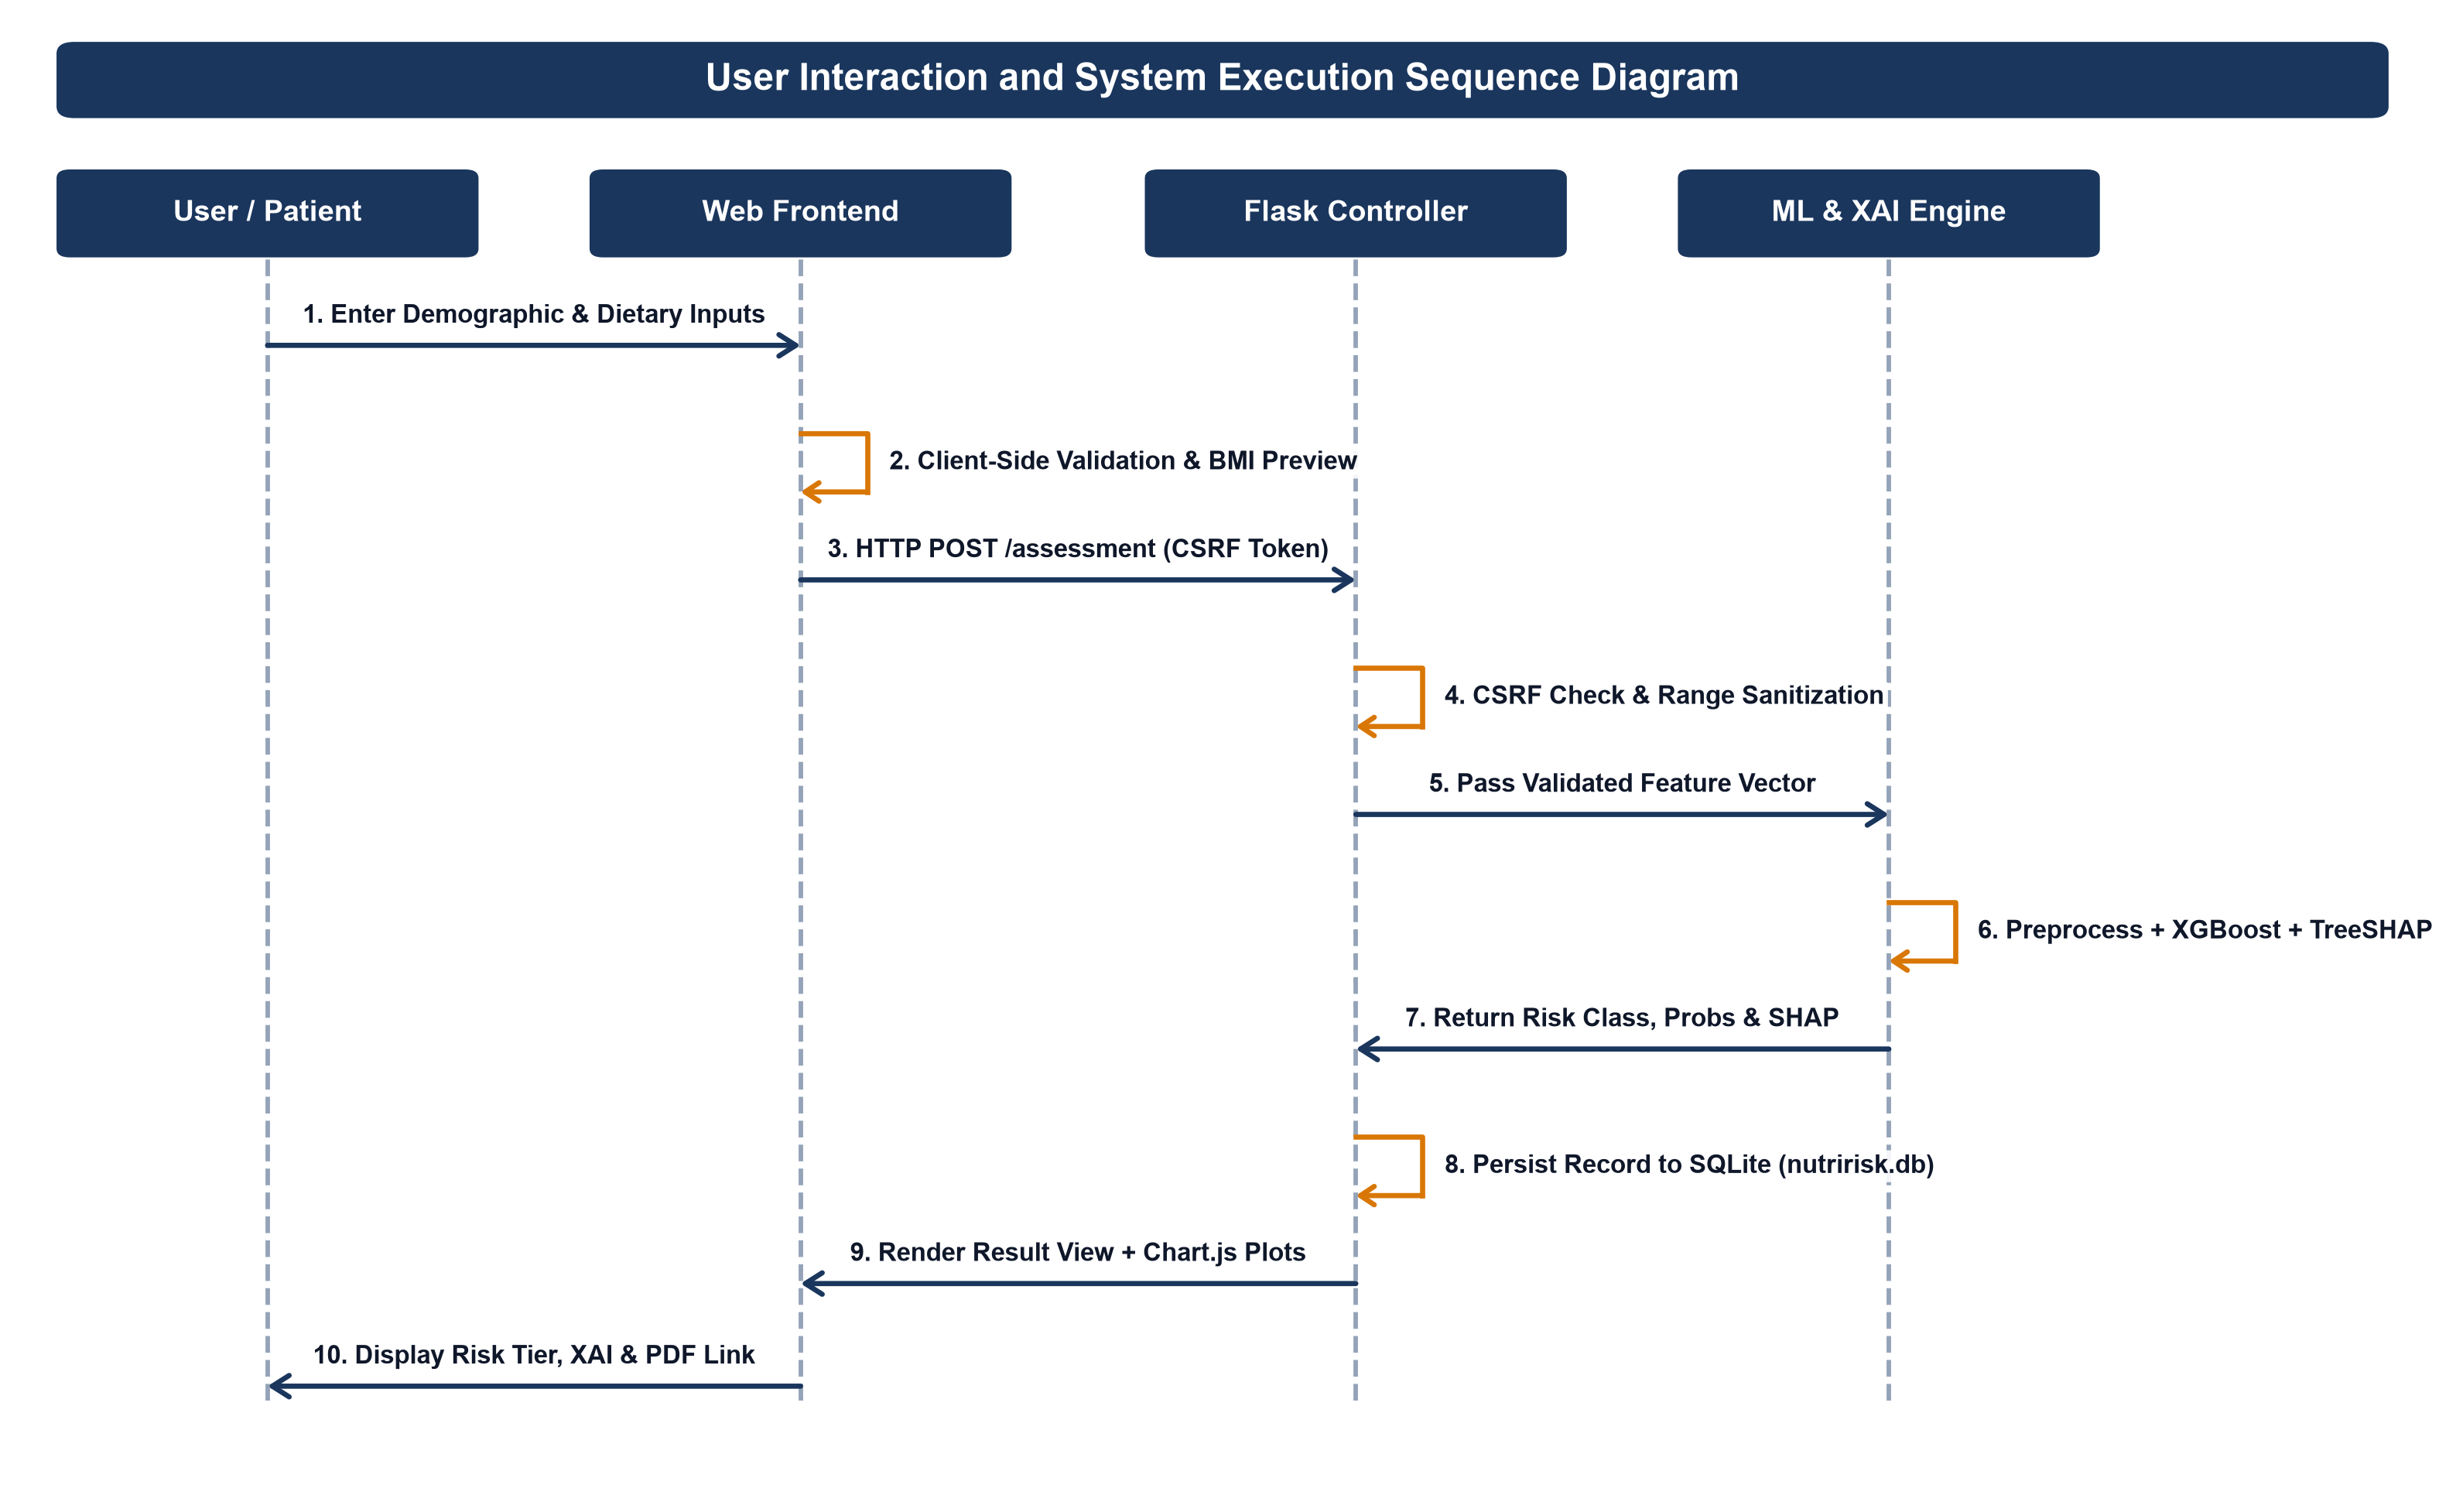
\includegraphics[width=\columnwidth]{figures/fig07_user_interaction.png}
\caption{Sequence diagram illustrating the authenticated user interaction lifecycle during clinical assessment and report export.}
\label{fig:seq}
\end{figure}

The database schema (Fig.~\ref{fig:db}) maintains referential integrity across five SQLite tables: \texttt{users} (credentials, Scrypt password hashes, and biometric face descriptors), \texttt{assessments} (clinical observations, calculated BMI, predicted risk level, probability vectors, and serialized SHAP summaries), \texttt{otp\_verifications} (2FA tokens), \texttt{admin\_audit\_logs} (immutable access logs), and \texttt{model\_metadata} (model governance records). 

Fig.~\ref{fig:seq} illustrates the complete sequence of user interaction, CSRF verification, pipeline execution, and report export. Furthermore, presenting class probabilities and feature contributions improves the interpretability of the model's predictions, allowing clinicians to inspect top contributing factors directly on screen or within exported PDF reports.

\section{Discussion}
\label{sec:discussion}
The experimental results demonstrate that combining non-invasive demographic indicators, dietary diversity indices, and anthropometrics enables preliminary nutritional risk stratification with strong predictive fidelity. XGBoost's empirical superiority over linear baselines ($+7.83\%$ accuracy, $+8.06\%$ Macro-F1) stems from its ability to model compounded, non-linear interactions—such as the elevated risk observed when poor dietary diversity coincides with advanced age and recent acute illness.

In primary care and community triage settings, the tool can collate basic information in under two minutes without expensive laboratory testing. The empirical verification of zero critical false negatives ($0$ High Risk cases classified as Low Risk) satisfies essential triage safety requirements. However, the model's ability to identify nutritional risk in real-world adult populations cannot be established without validation using independent clinical data. The tool serves as a clinical decision-support prototype rather than an autonomous diagnostic system.

\section{Limitations and Future Work}
\label{sec:limitations}
Several limitations must be acknowledged:
\begin{enumerate}
    \item \textbf{Synthetic Data Boundary:} Although the dataset was calibrated against international survey distributions, synthetic records may not fully reflect the biological variance, measurement error, or comorbidities of hospitalized patients.
    \item \textbf{Adult Population Scope:} The framework is restricted to individuals aged 18 years and above; pediatric cohorts require distinct anthropometric Z-score models (WHO child growth standards).
    \item \textbf{Cross-Sectional Limitation:} The current model evaluates a single temporal snapshot and does not capture longitudinal trajectories of weight loss.
\end{enumerate}

Future work will focus on validating the framework using real-world public health survey datasets (such as NFHS-5), incorporating longitudinal weight tracking, conducting prospective clinical validation trials in primary care centers, and porting the inference engine to lightweight on-device formats (ONNX/TFLite) for offline deployment in rural health posts.

\section{Conclusion}
\label{sec:conclusion}
This paper presented \textbf{NutriRisk AI}, a machine-learning-based framework for preliminary nutritional risk stratification in adults. The application processes demographic, anthropometric, dietary, lifestyle, socioeconomic, and recent health-related information, calculates BMI from height and weight ($\text{kg/m}^2$), and classifies individuals into Low-, Moderate-, or High-Risk categories. Benchmarked across five supervised algorithms on $6{,}000$ calibrated records, our optimized XGBoost pipeline achieved champion performance ($78.50\%$ accuracy, $78.83\%$ Macro-F1, $0.9241$ ROC-AUC, and zero critical false negatives). By integrating game-theoretic TreeSHAP interpretability and occlusion sensitivity into a secure, production-grade web application with automated clinical reporting, the system demonstrates a viable engineering approach for accessible nutritional screening. Future research will focus on prospective clinical validation and integration into primary healthcare workflows.

\bibliographystyle{IEEEtran}
\bibliography{references}

\end{document}
